\documentclass[12pt]{article}
\usepackage{graphicx}
\usepackage{float}
\usepackage{subcaption}

%
% Title.
\title{EE236: Experiment 7\\
Solar cell C-V profiing}

% Author
\author{Aaron John Sabu, 170070050}

% begin the document.
\begin{document}

% make a title page.
\maketitle

\section{Aim of the experiment}

The primary goal of this experiment is to design a simple op-amp based circuit to measure capacitance of a pn junction. The circuit is used to measure the voltage dependence of a pn junction (solar cell) capacitance. The secondary goal of this experiment is to use the C-V profile measurements to estimate the doping density and built-in potential of the solar cell.

\section{Observations and inferences}

The solar cell box used by the group is shown below:
\begin{figure}[H]
	\centering
	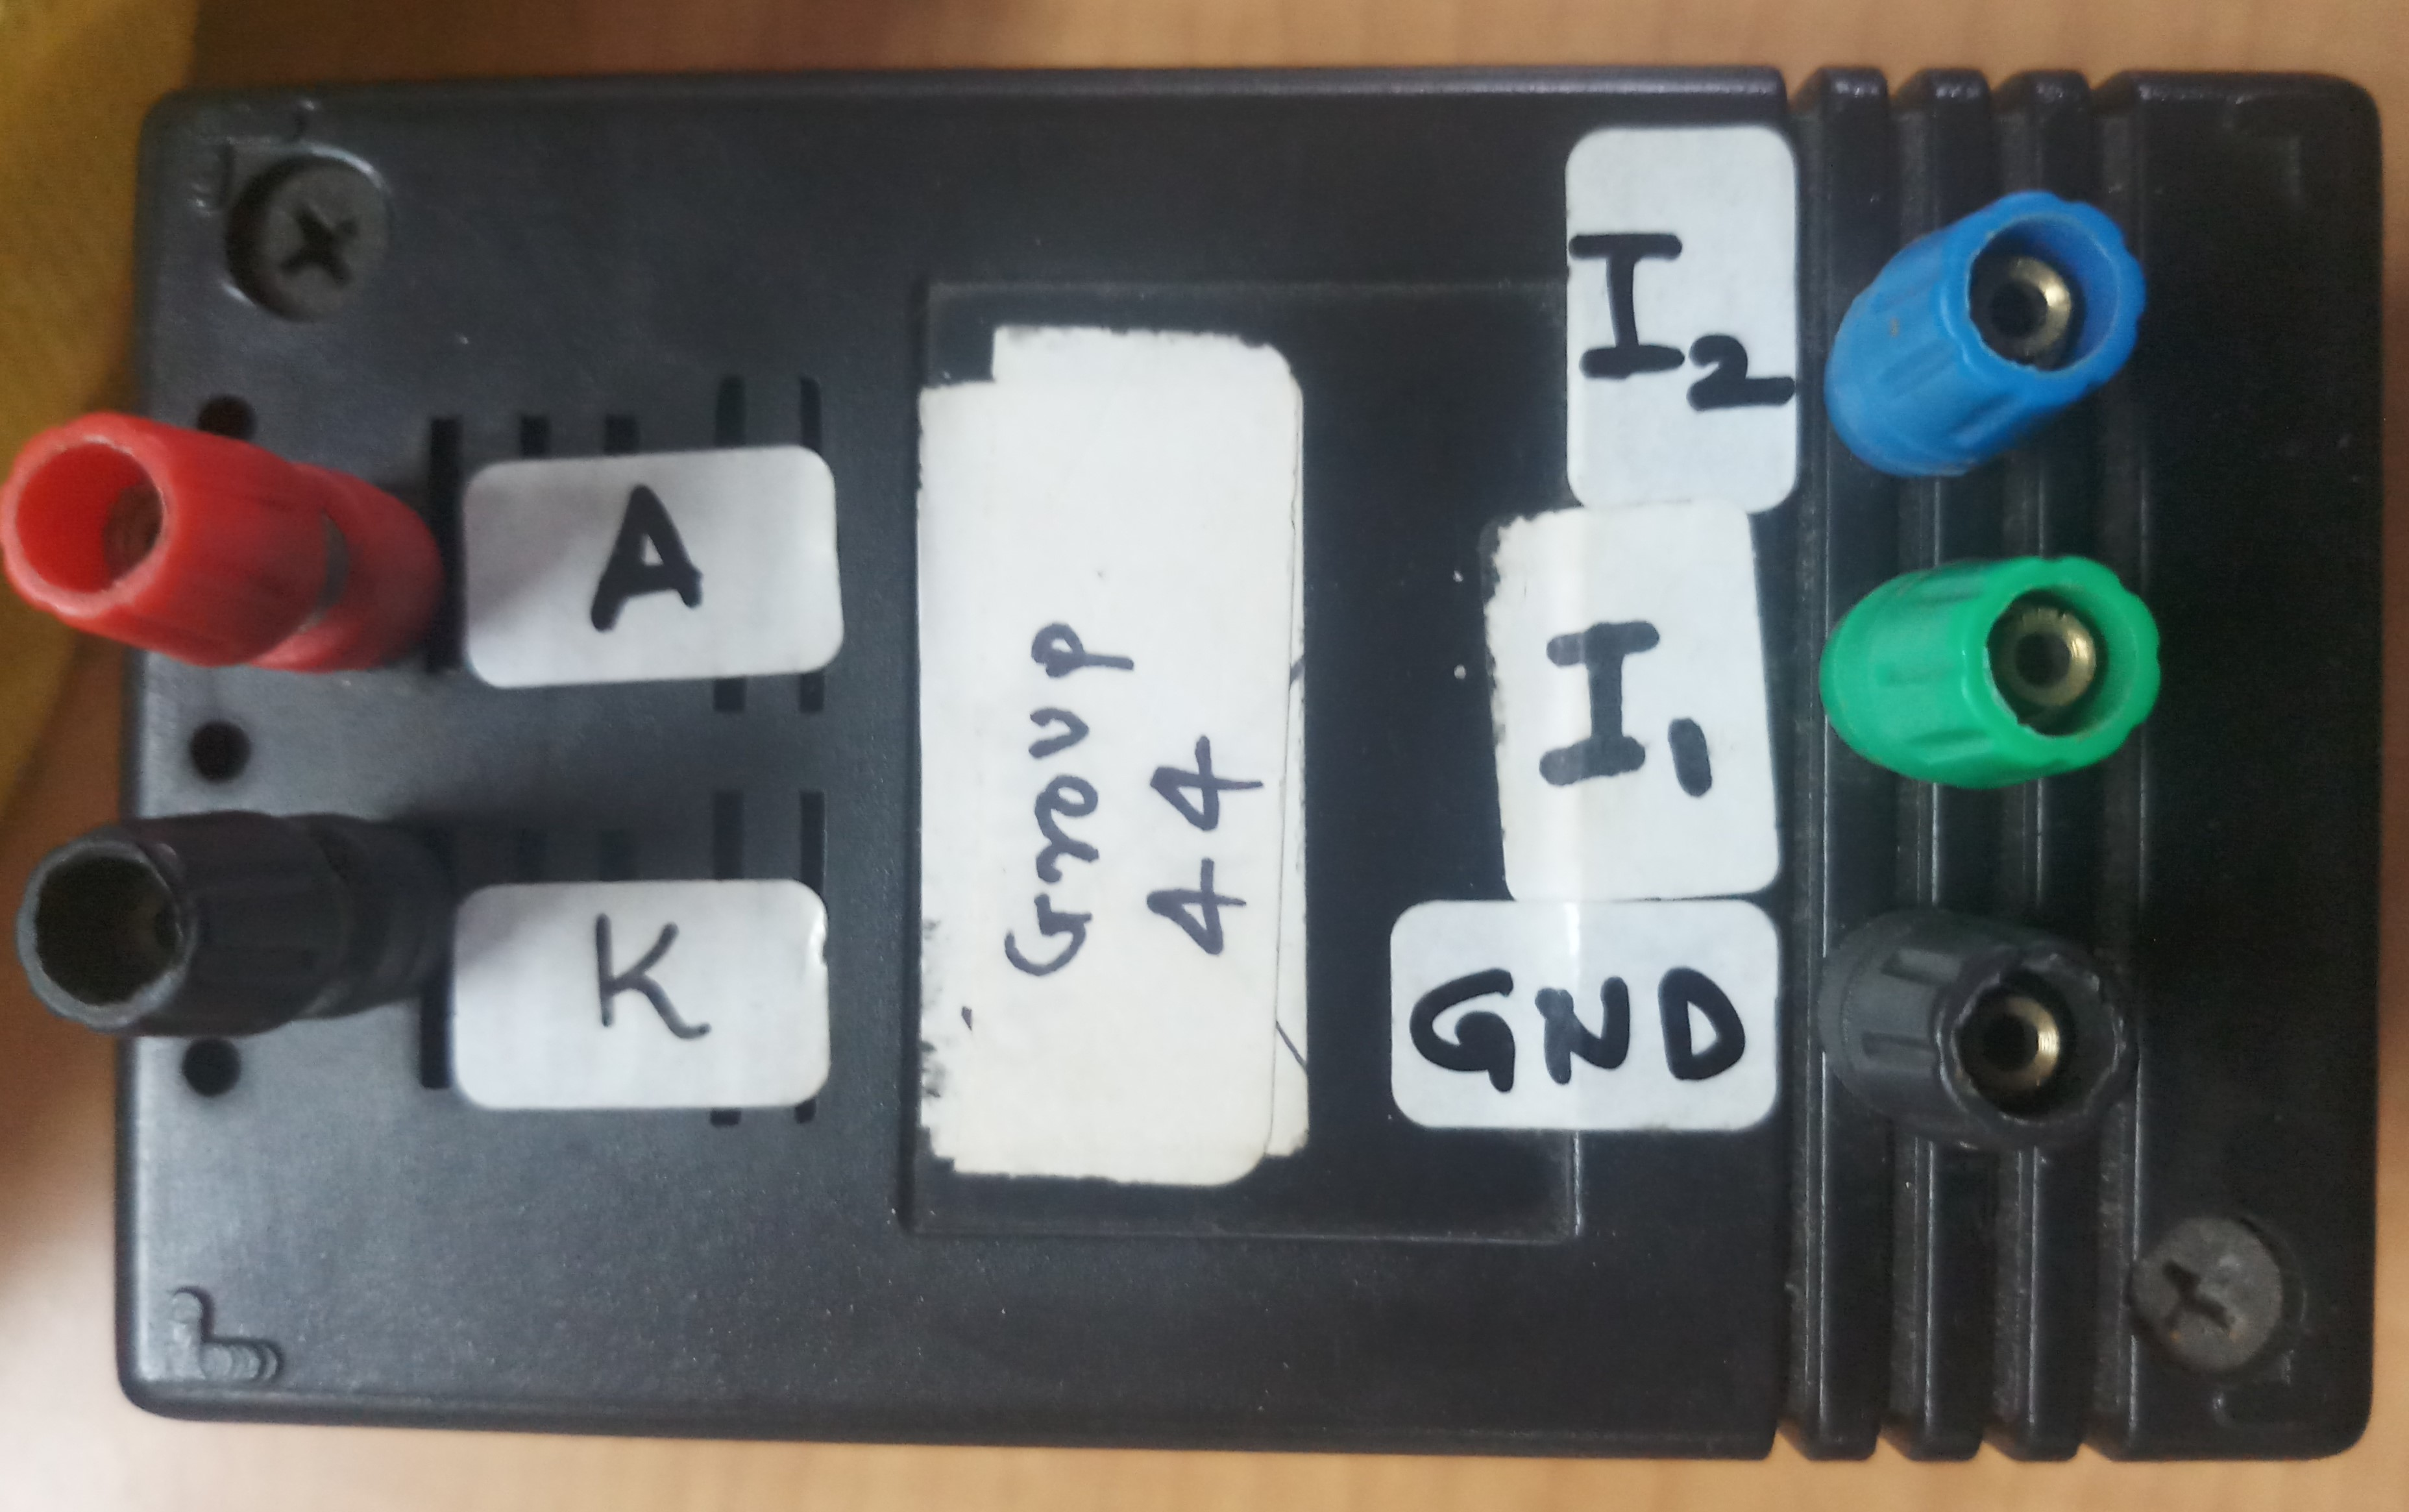
\includegraphics[scale=0.06]{SolarCellBox.jpg}
	\caption{Solar Cell Box}
\end{figure}

\subsection{Part A}
\begin{figure}[H]
	\begin{subfigure}[b]{0.5\linewidth}
		\centering
		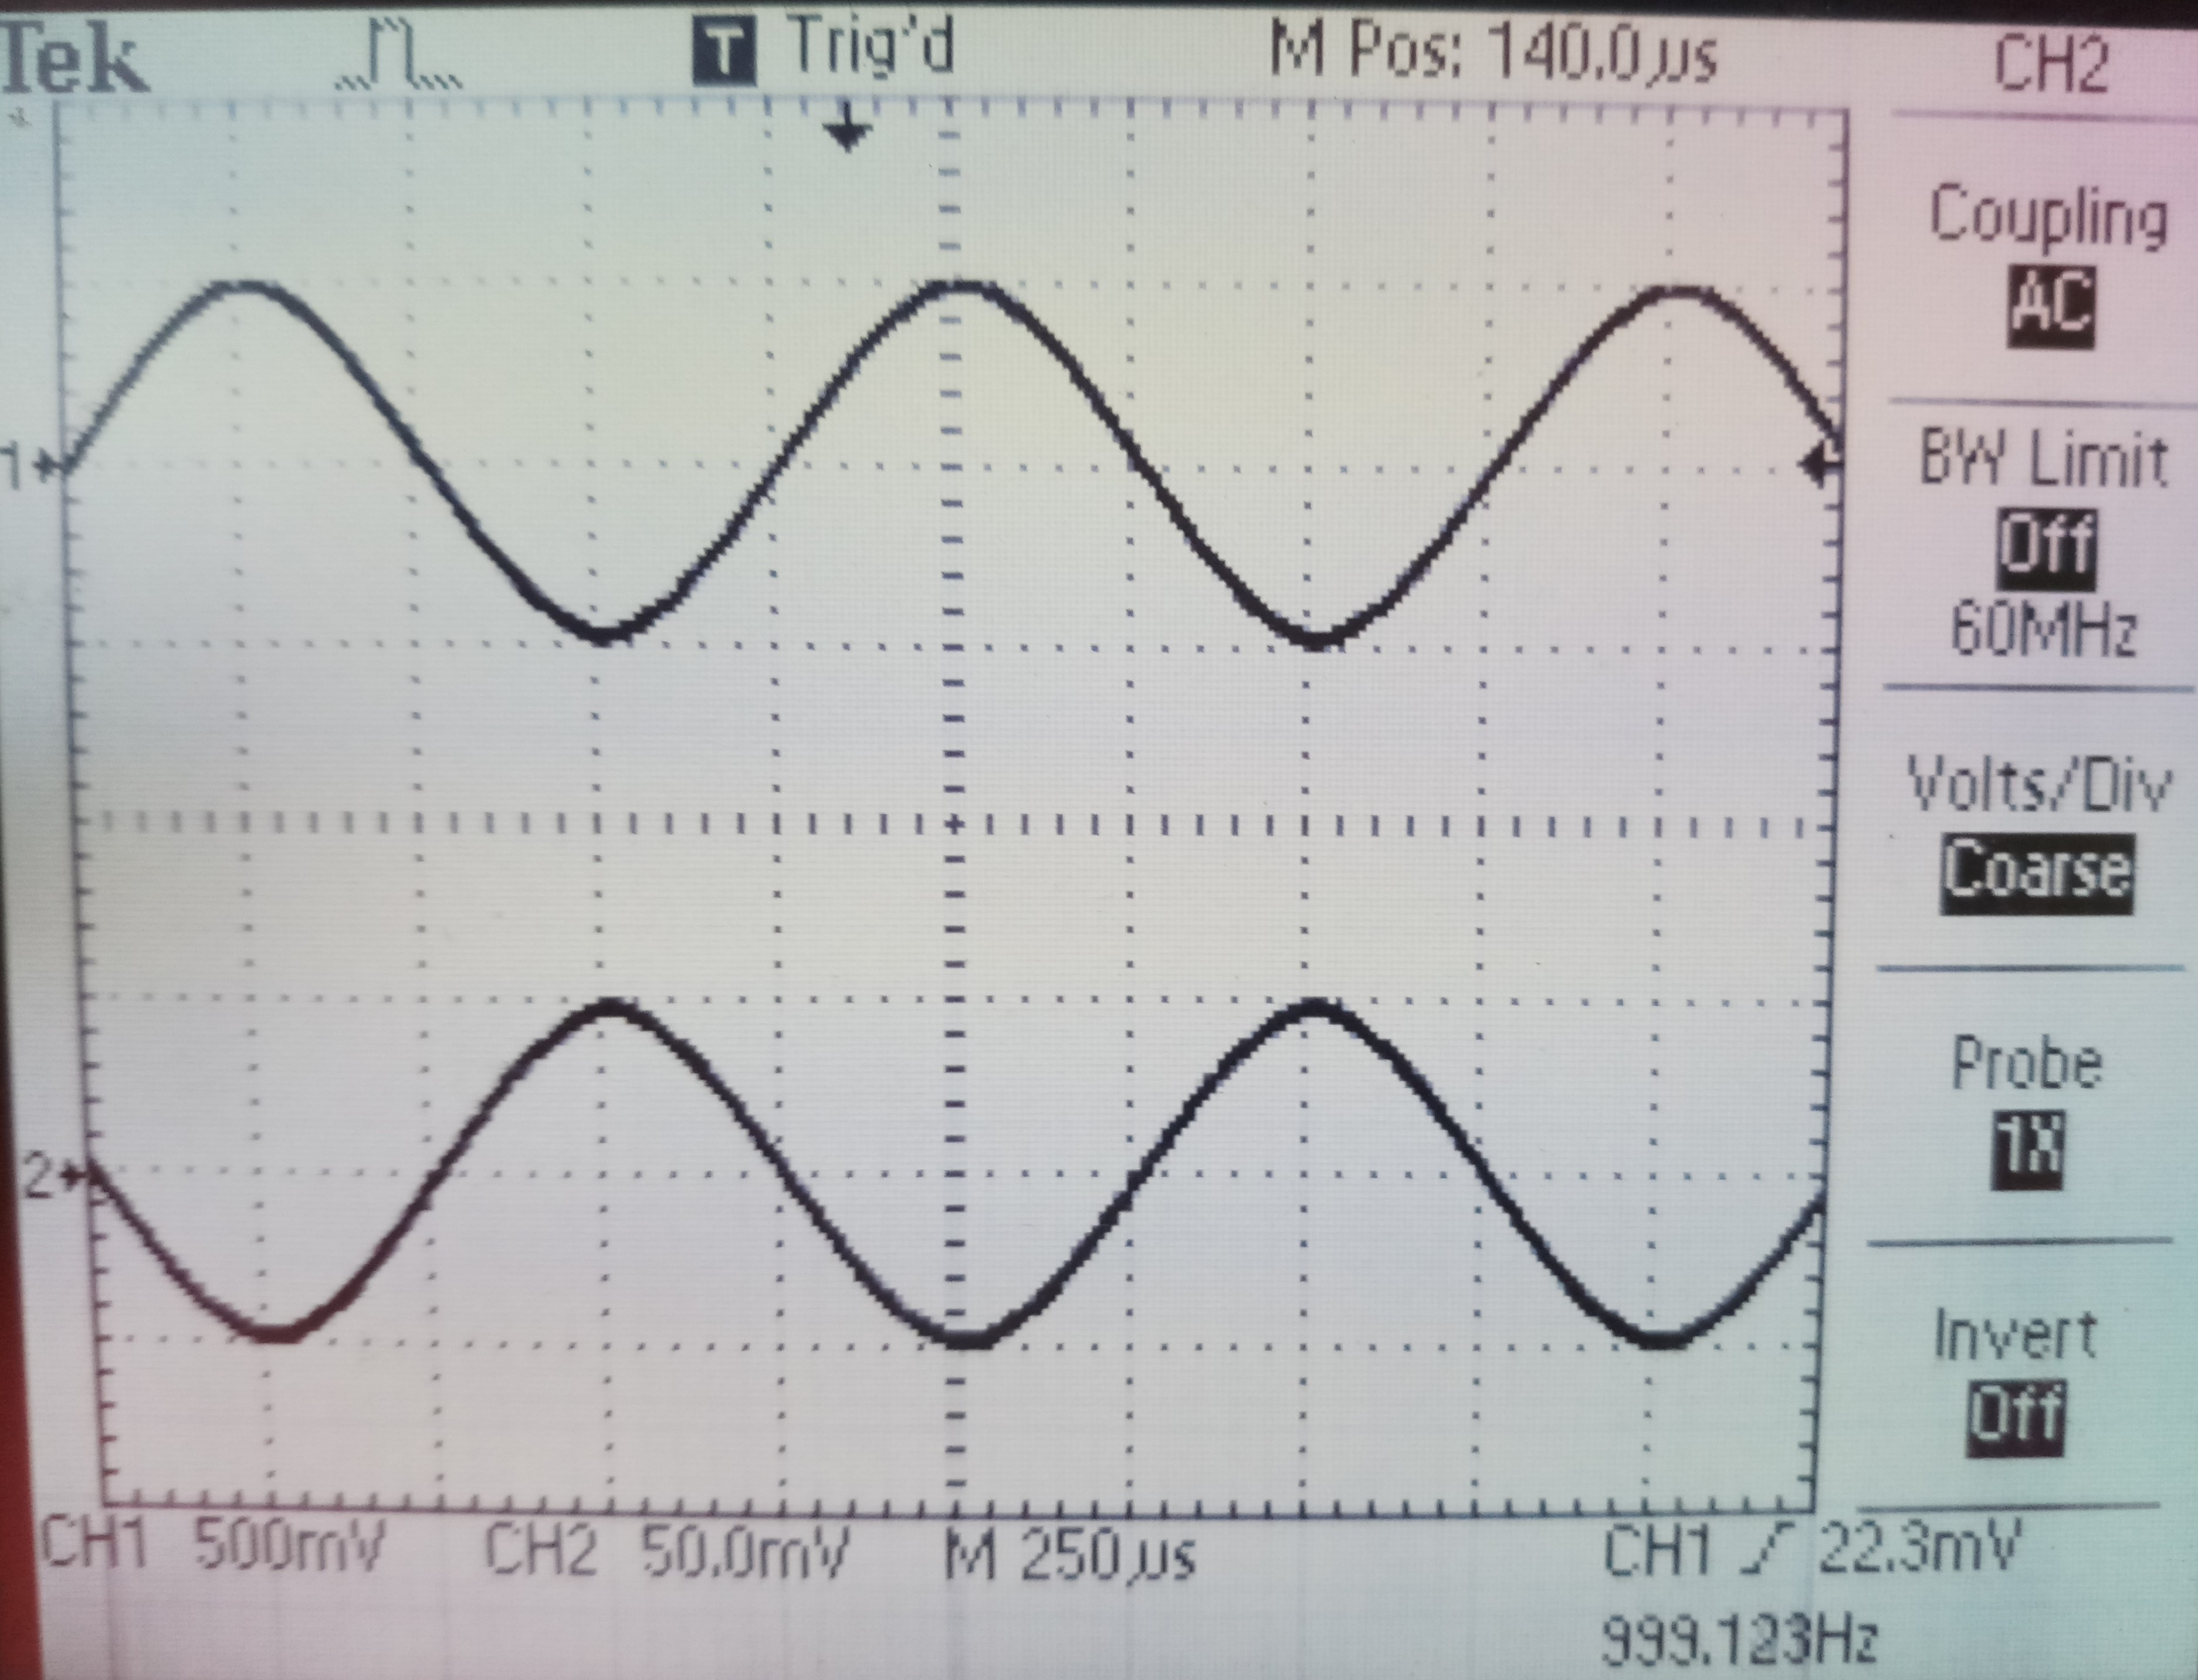
\includegraphics[width = \linewidth]{PartA_AC.jpg}
		\caption{AC Coupling of Output}
	\end{subfigure}
	\begin{subfigure}[b]{0.5\linewidth}
		\centering
		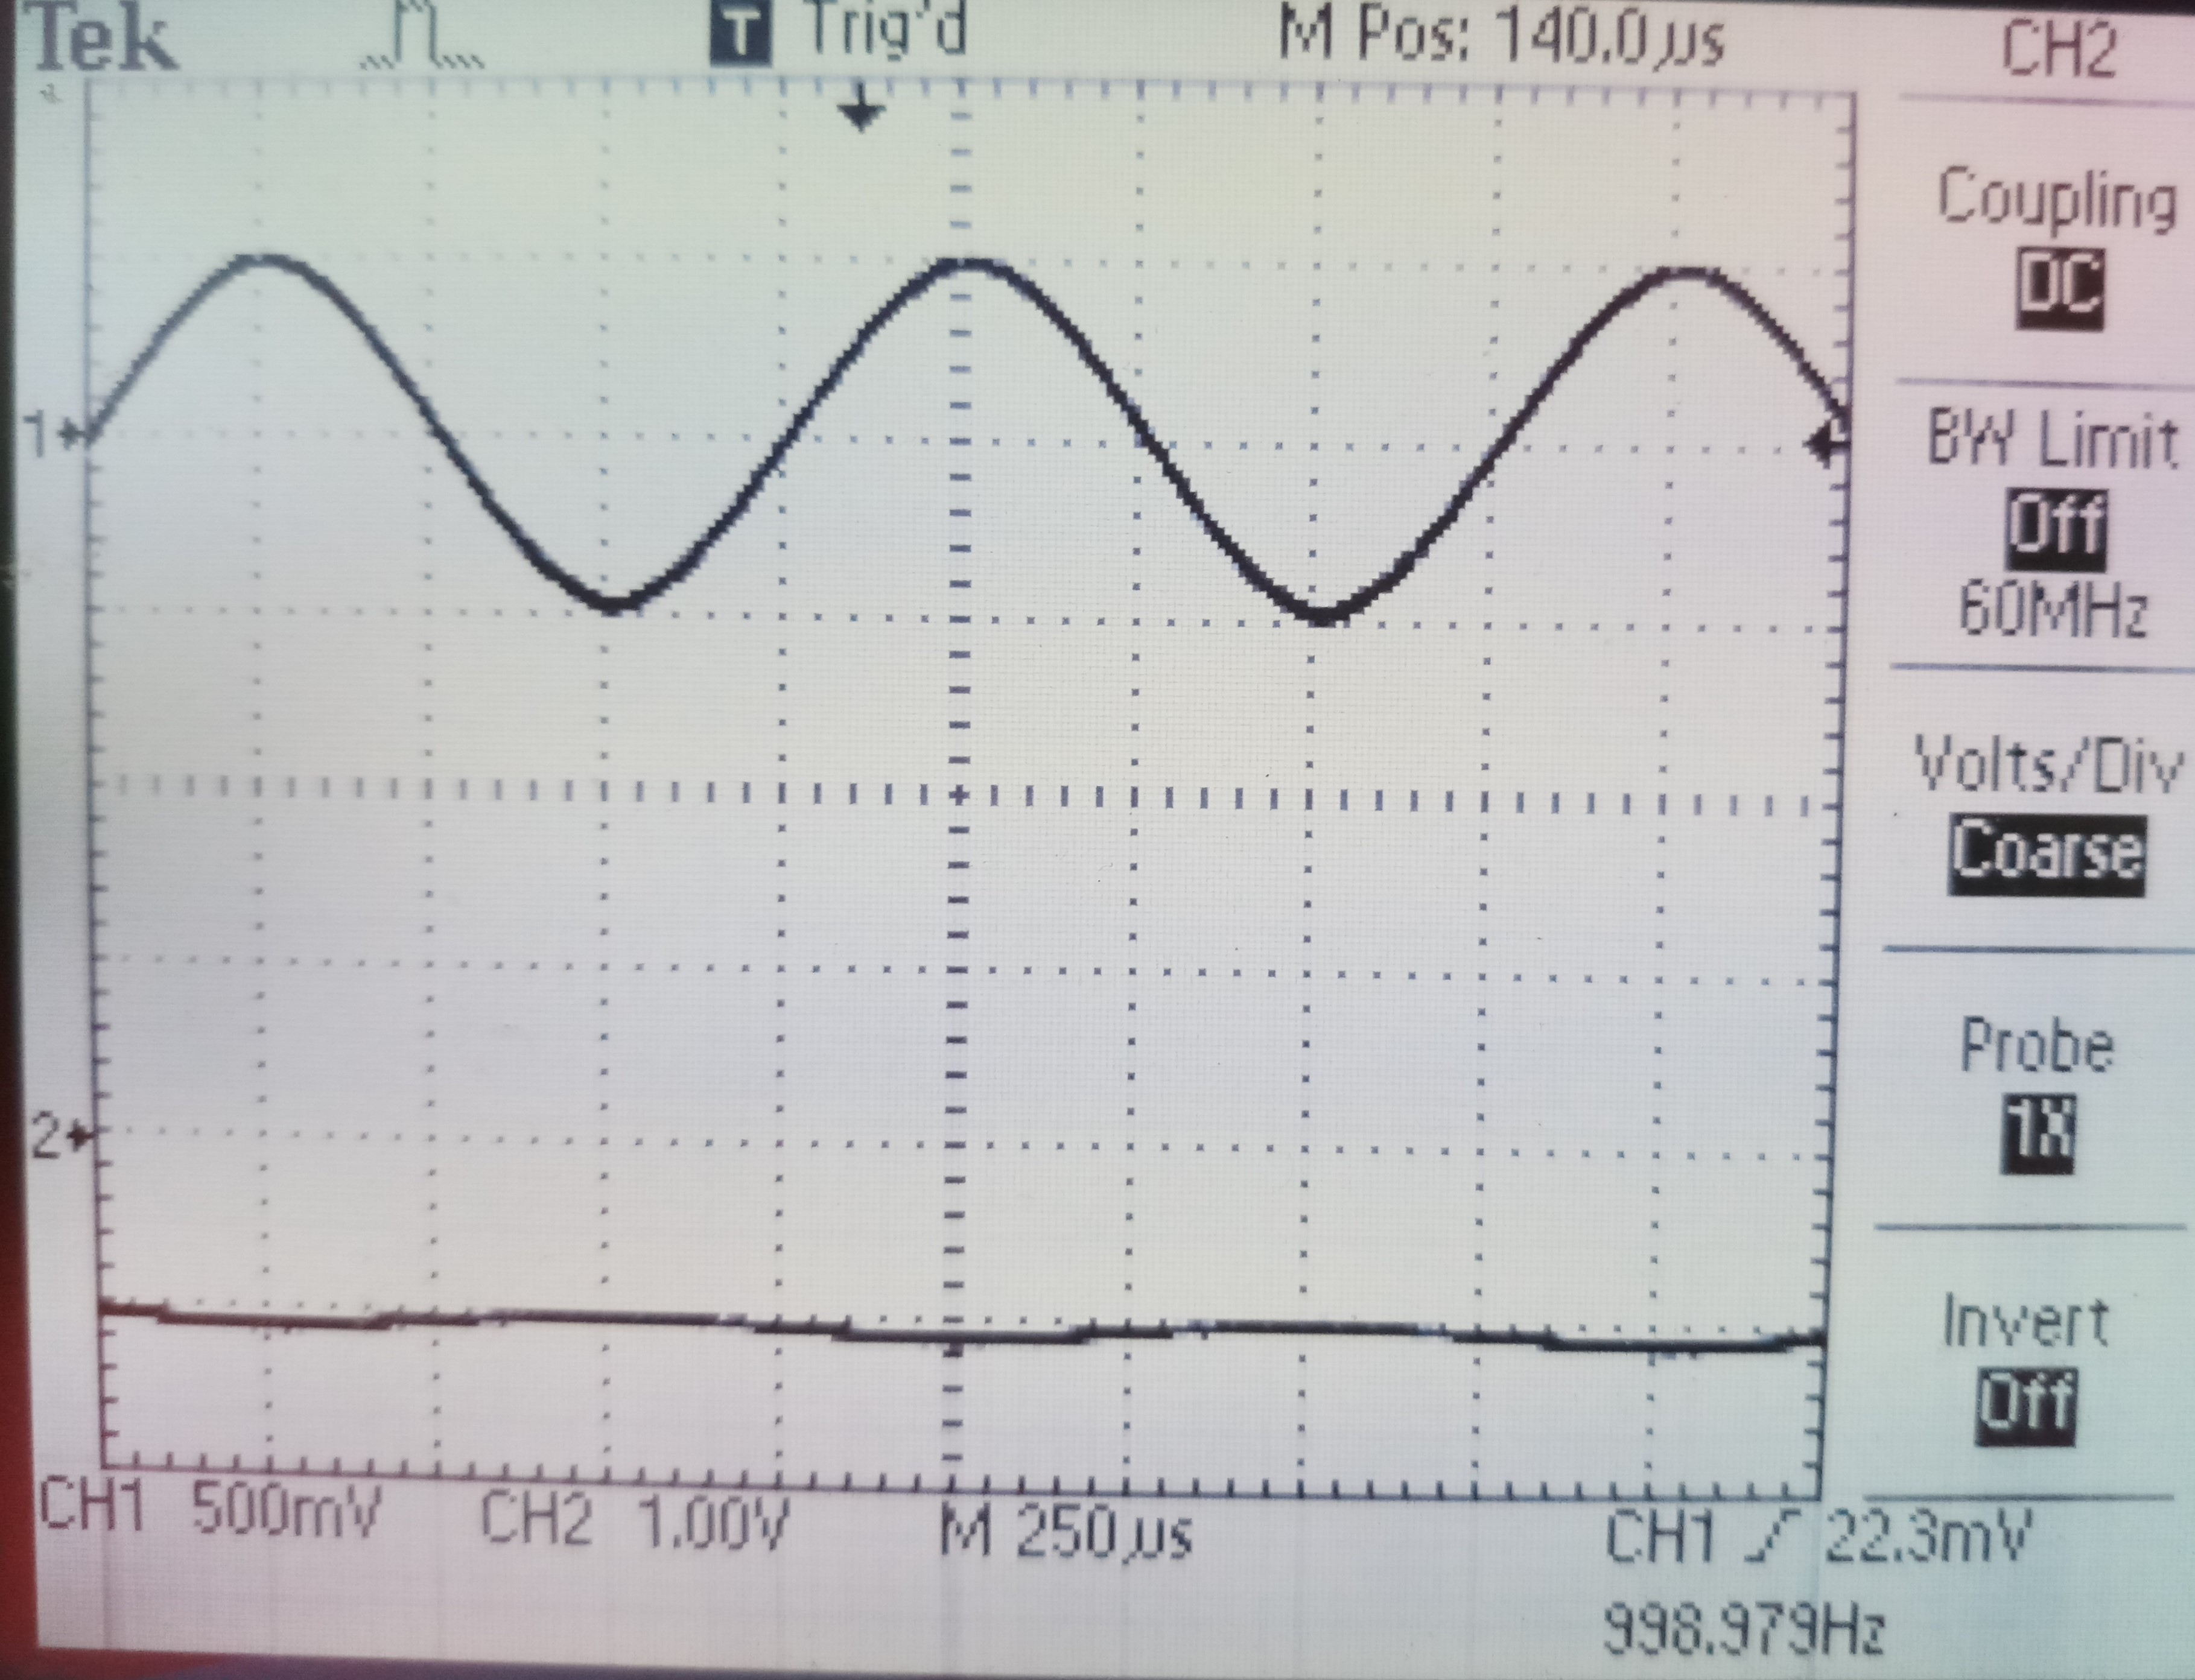
\includegraphics[width = \linewidth, trim = {0 0 0 0}, clip]{PartA_DC.jpg}
		\caption{DC Coupling of Output}
	\end{subfigure}
	\caption{Part A - Outputs}
\end{figure}
As is visible, the input voltages have been summed up and the negated form is given as output. Hence the summing amplifier has functioned properly.
\[ V_{DUT} = -R_F \left( \frac{V_{dc}}{R_2} + \frac{V_{ac}}{R_1} \right) \] \[ V_{DUT} = - \left( V_{dc} + \frac{V_{ac}}{10} \right) \]

\subsection{Part B}
\begin{figure}[H]
	\begin{subfigure}[b]{0.5\linewidth}
		\centering
		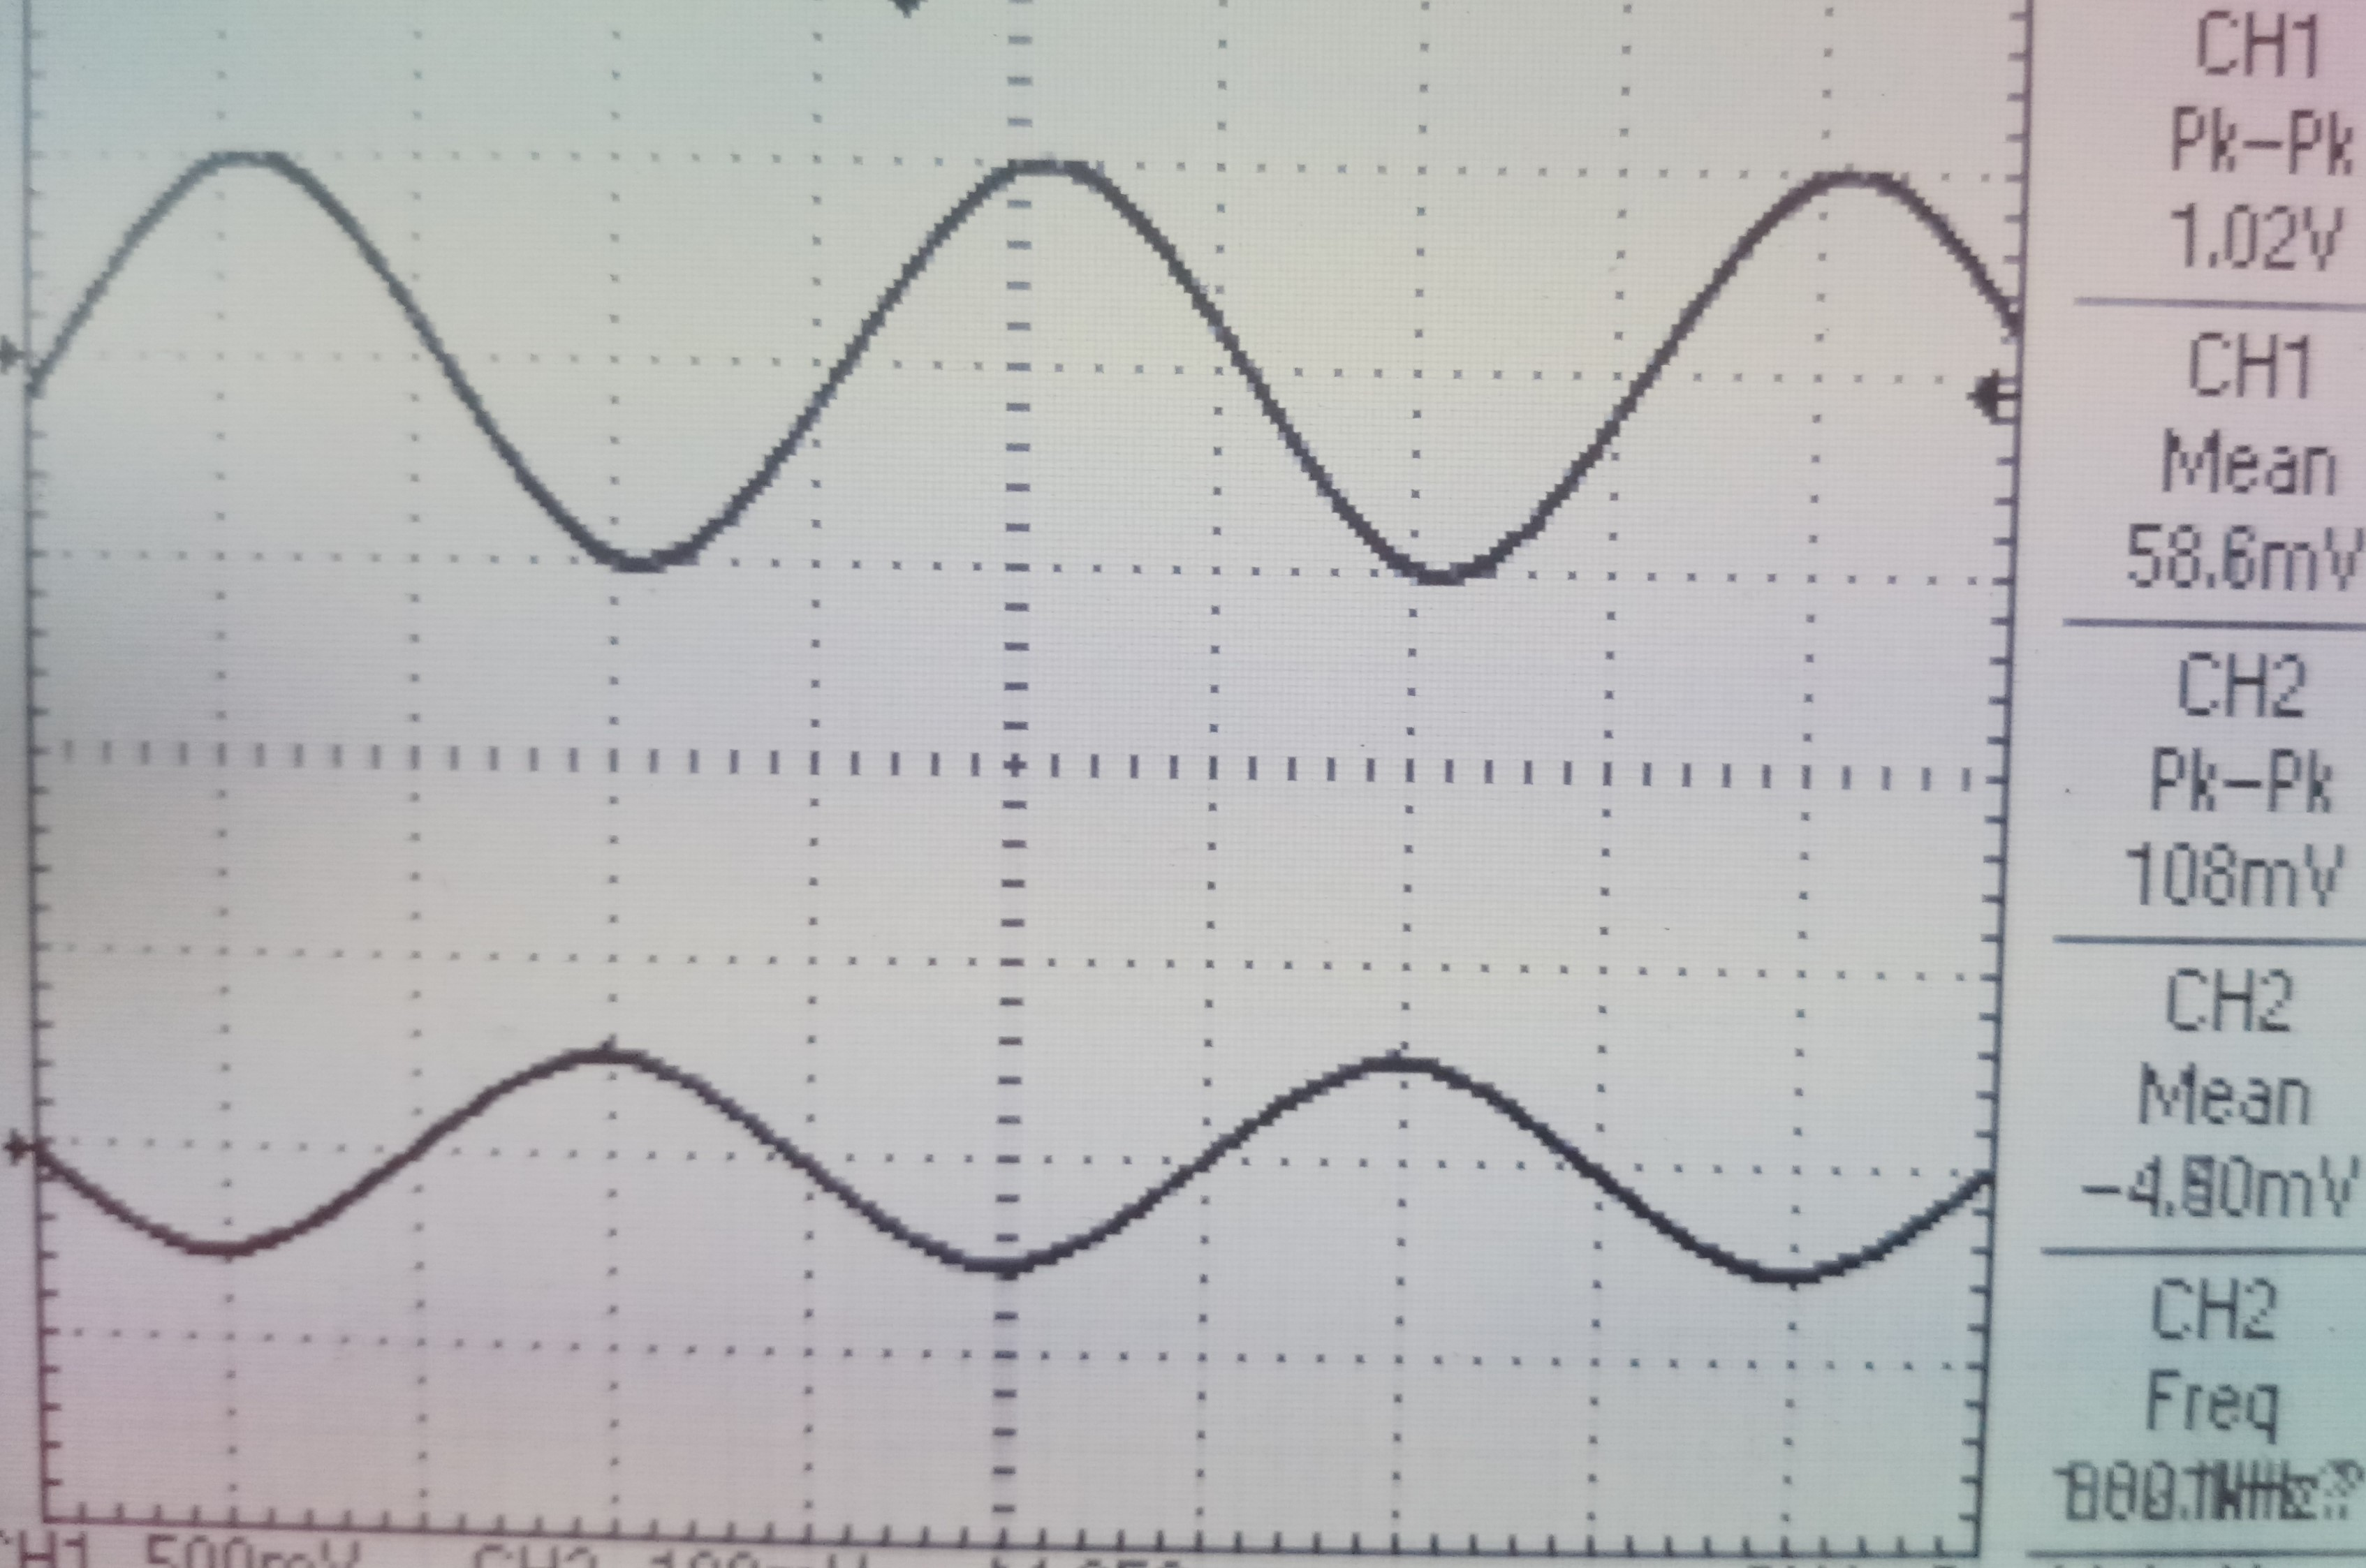
\includegraphics[width = \linewidth, trim = {0 0 0 0}, clip]{PartB_AC.jpg}
		\caption{AC Coupling of Output}
	\end{subfigure}
	\begin{subfigure}[b]{0.5\linewidth}
		\centering
		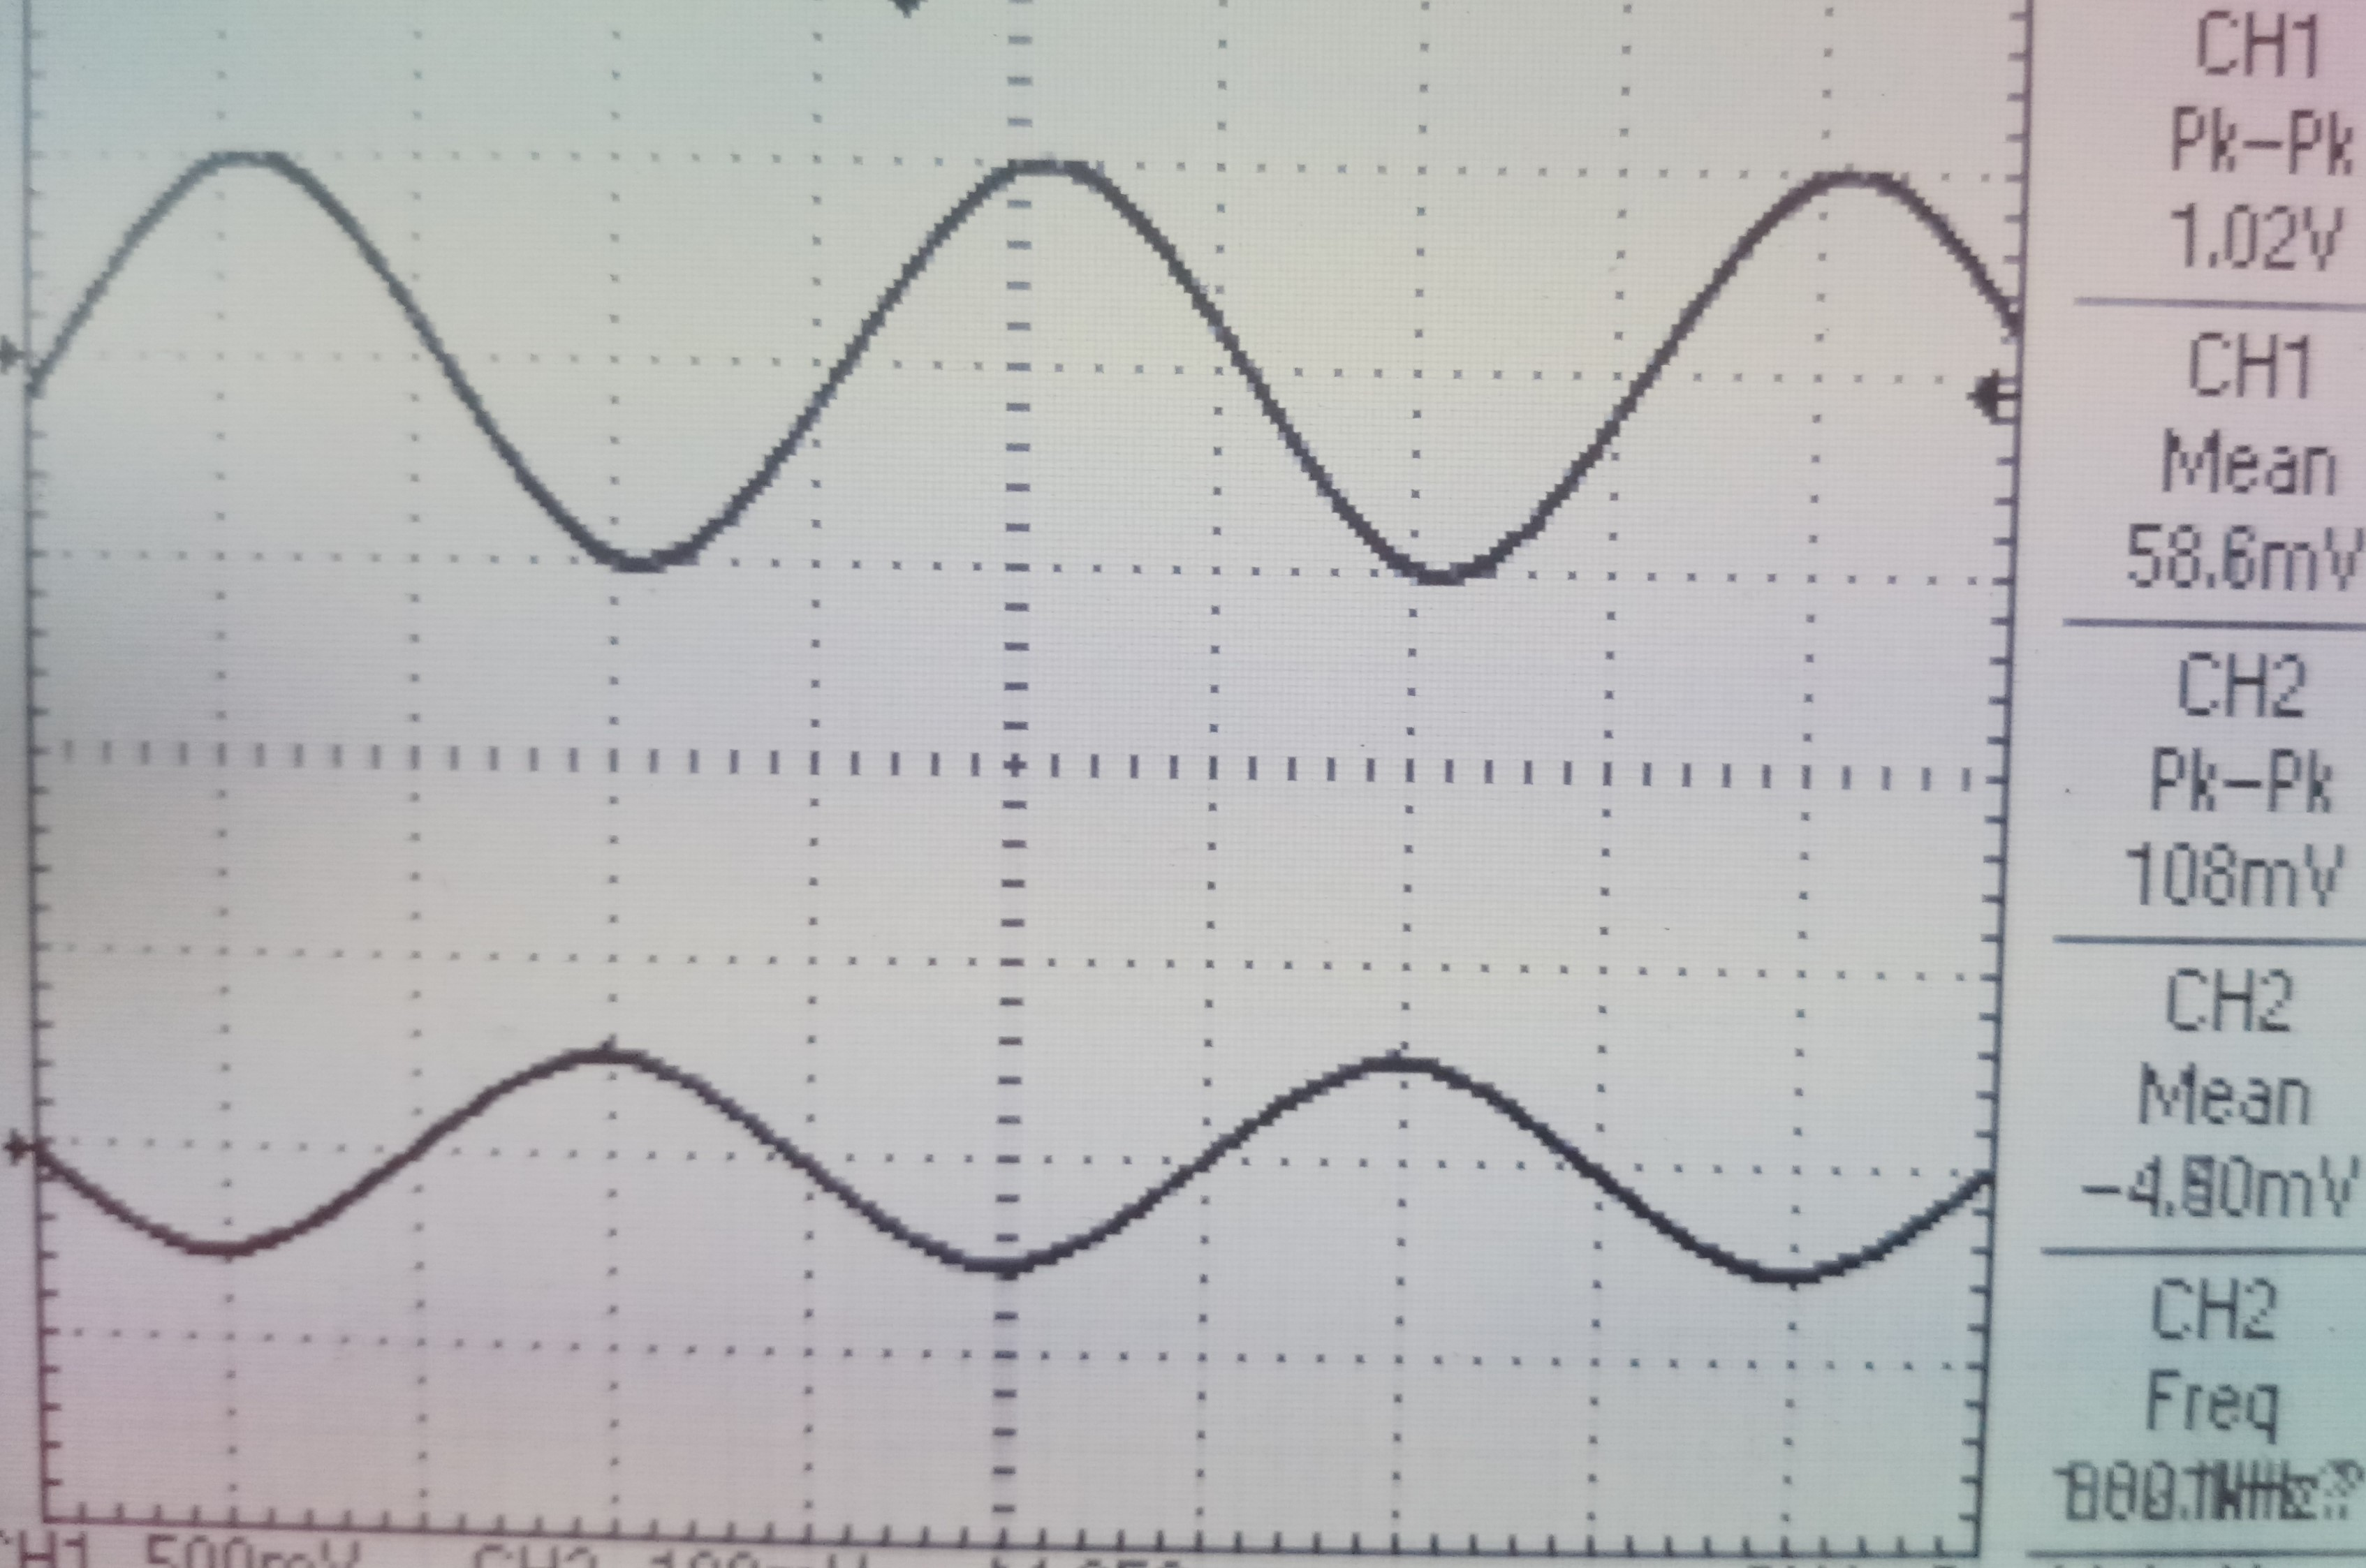
\includegraphics[width = \linewidth, trim = {0 0 0 0}, clip]{PartB_AC.jpg}
		\caption{DC Coupling of Output}
	\end{subfigure}
	\caption{Part B - Outputs}
\end{figure}
\[ V_{out} = -V_{DUT}\left( \frac{Z_{fb}}{Z_{DUT}} \right) \] Since the capacitance reactance of the capacitor is very large when compared to the resistor, we get: \[ R_{DUT} = R_{fb}\left( \frac{-V_{DUT_{p-p}}}{V_{out_{p-p}}} \right) \] \[ R_{DUT} = 10 k\Omega \times \left( \frac{108}{1020} \right) \approx 1k\Omega \]


\subsection{Part C}
\begin{figure}[H]
	\centering
	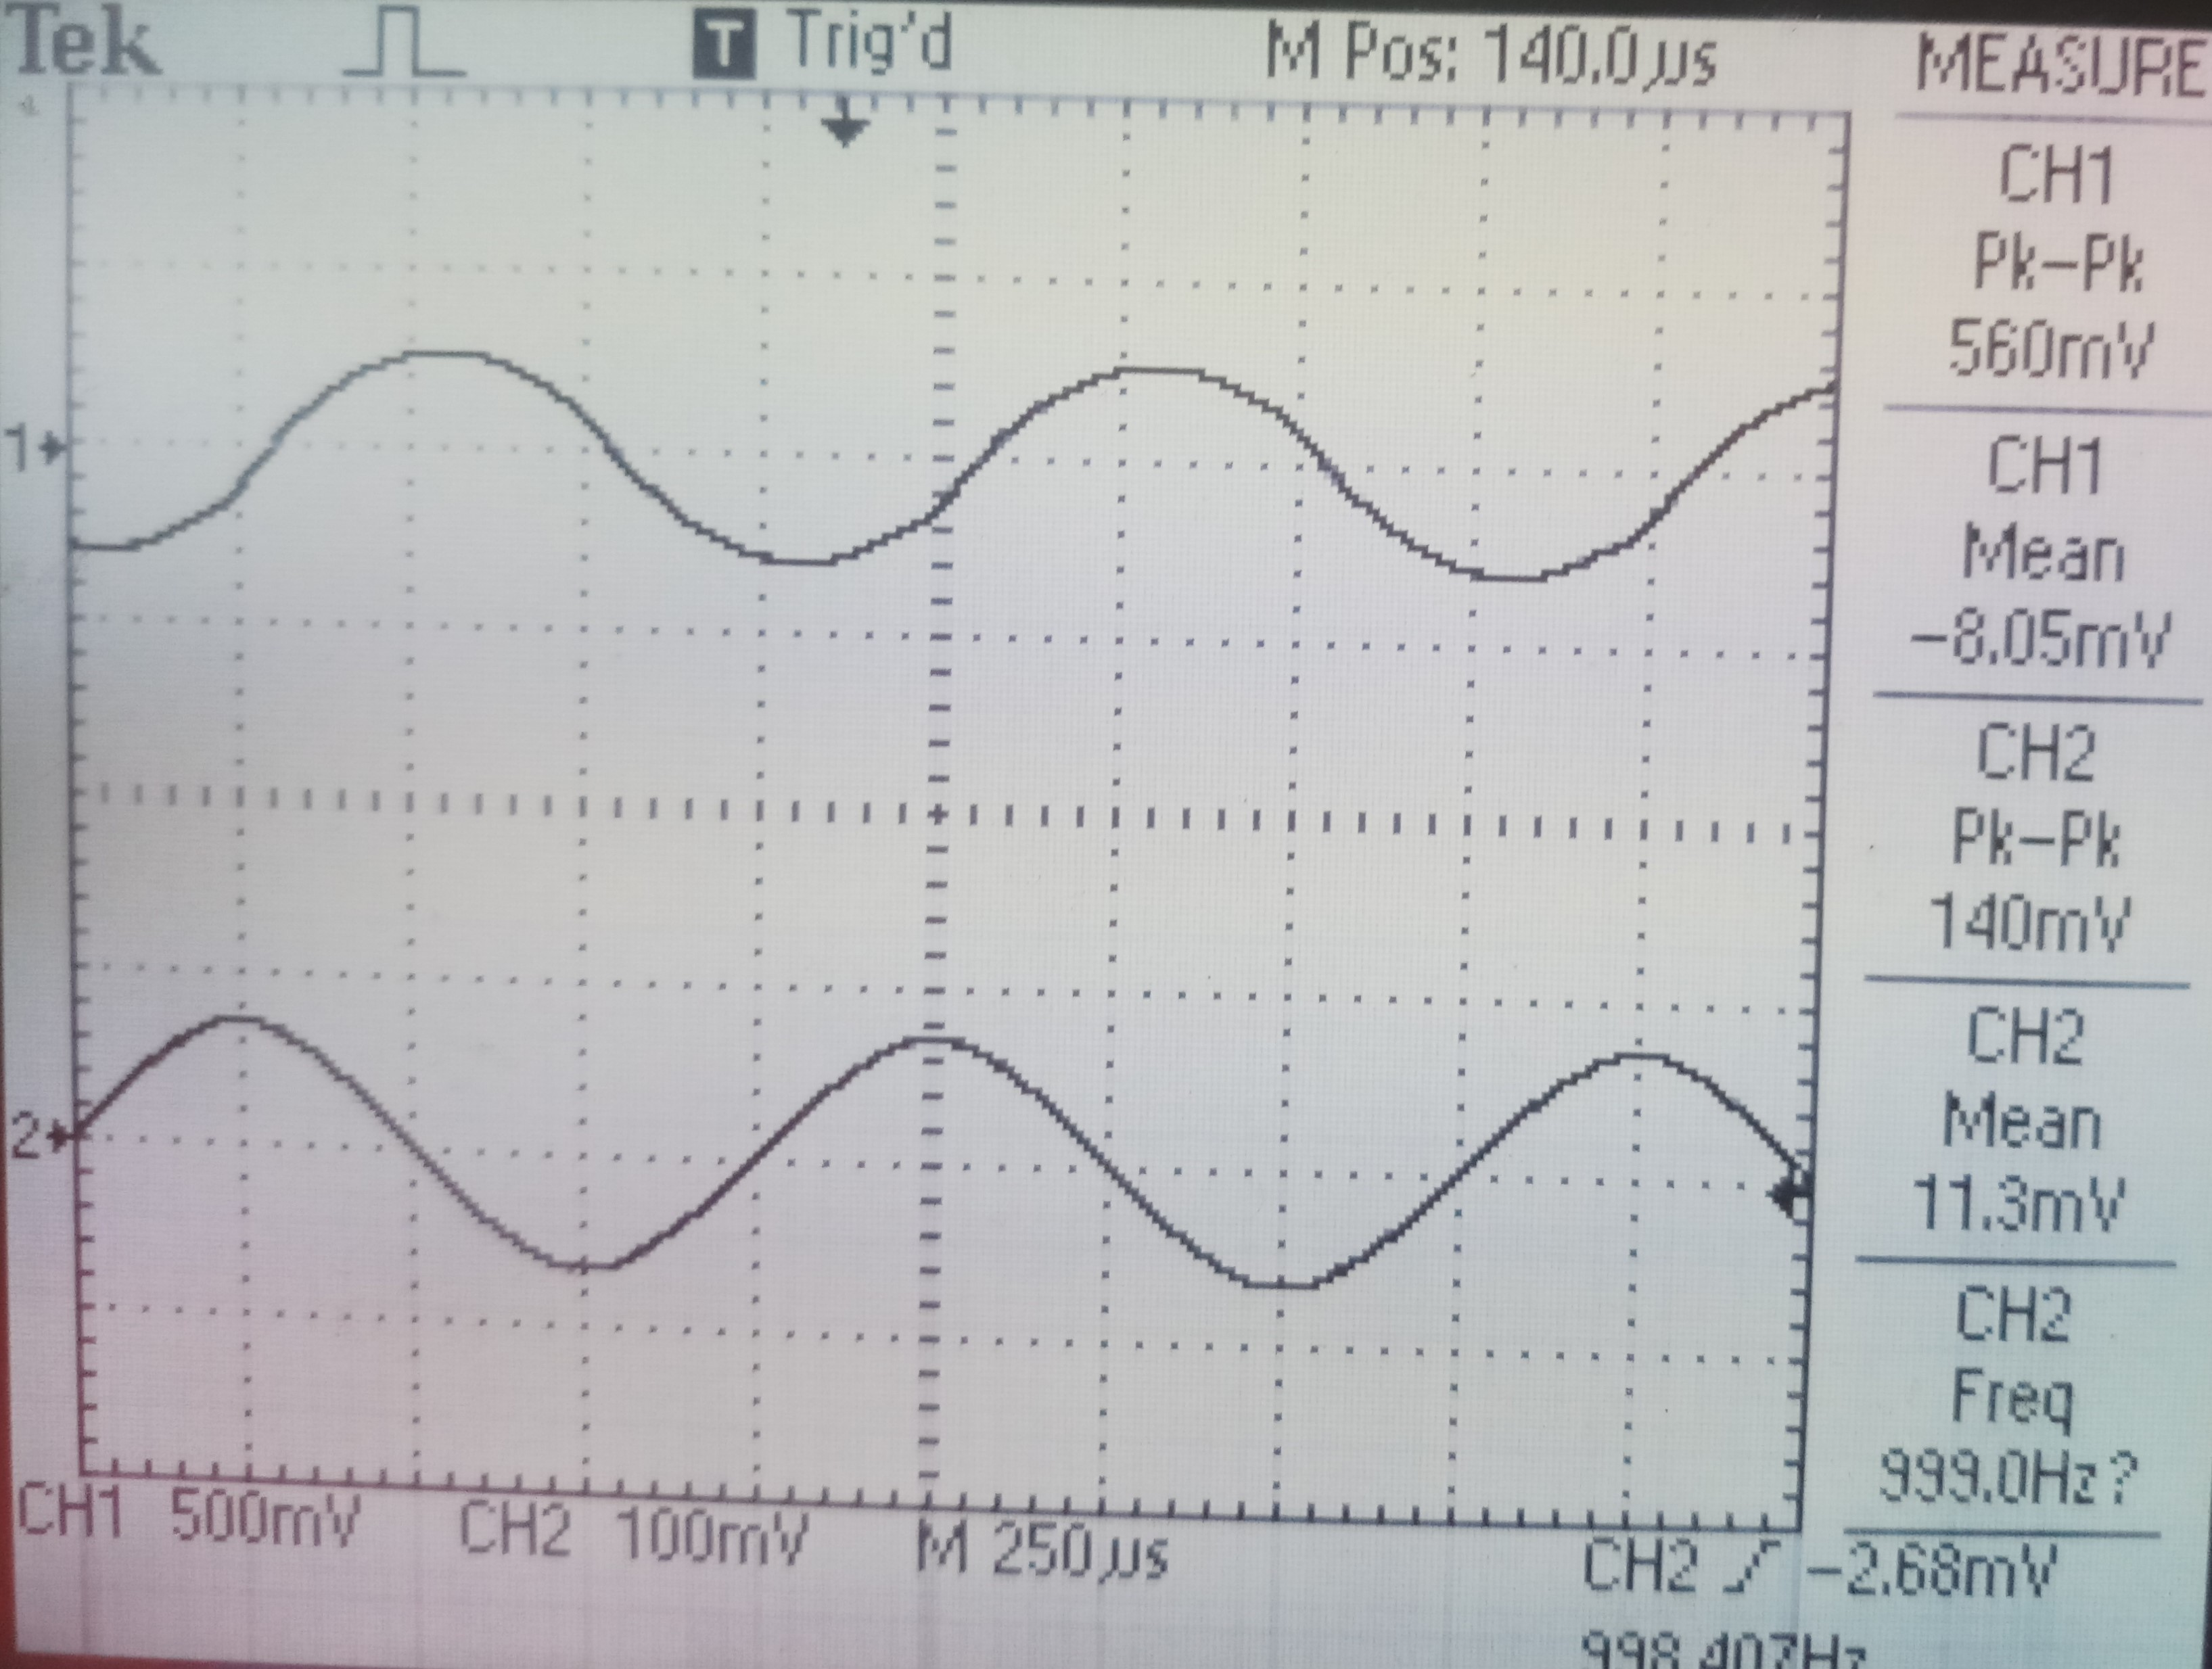
\includegraphics[scale=0.08]{PartC.jpg}
	\caption{Part C - Output}
\end{figure}
\[ V_{out} = -V_{DUT}\left( \frac{Z_{fb}}{Z_{DUT}} \right) \] \[ C_{DUT} = \left( \frac{- V_{out_{p-p}}}{Z_{fb} \times \omega \times V_{DUT_{p-p}}} \right) \] \[ C_{DUT} = \left(  \frac{560}{7723 \times 2 \pi \times 998 \times 140} \right) = 82.6\ \mu F \] 
Though it can be observed that the value of capacitance we obtained was not equal to the marked capacitance, it is also observed from the LCR meter that the real capacitance did not match the marked capacitance. In fact the real capacitance was \( C_{REAL} = 78.6\ \mu F \) which almost matched our result \( C_{MEAS} = 82.6\ \mu F \).
\begin{figure}[H]
	\centering
	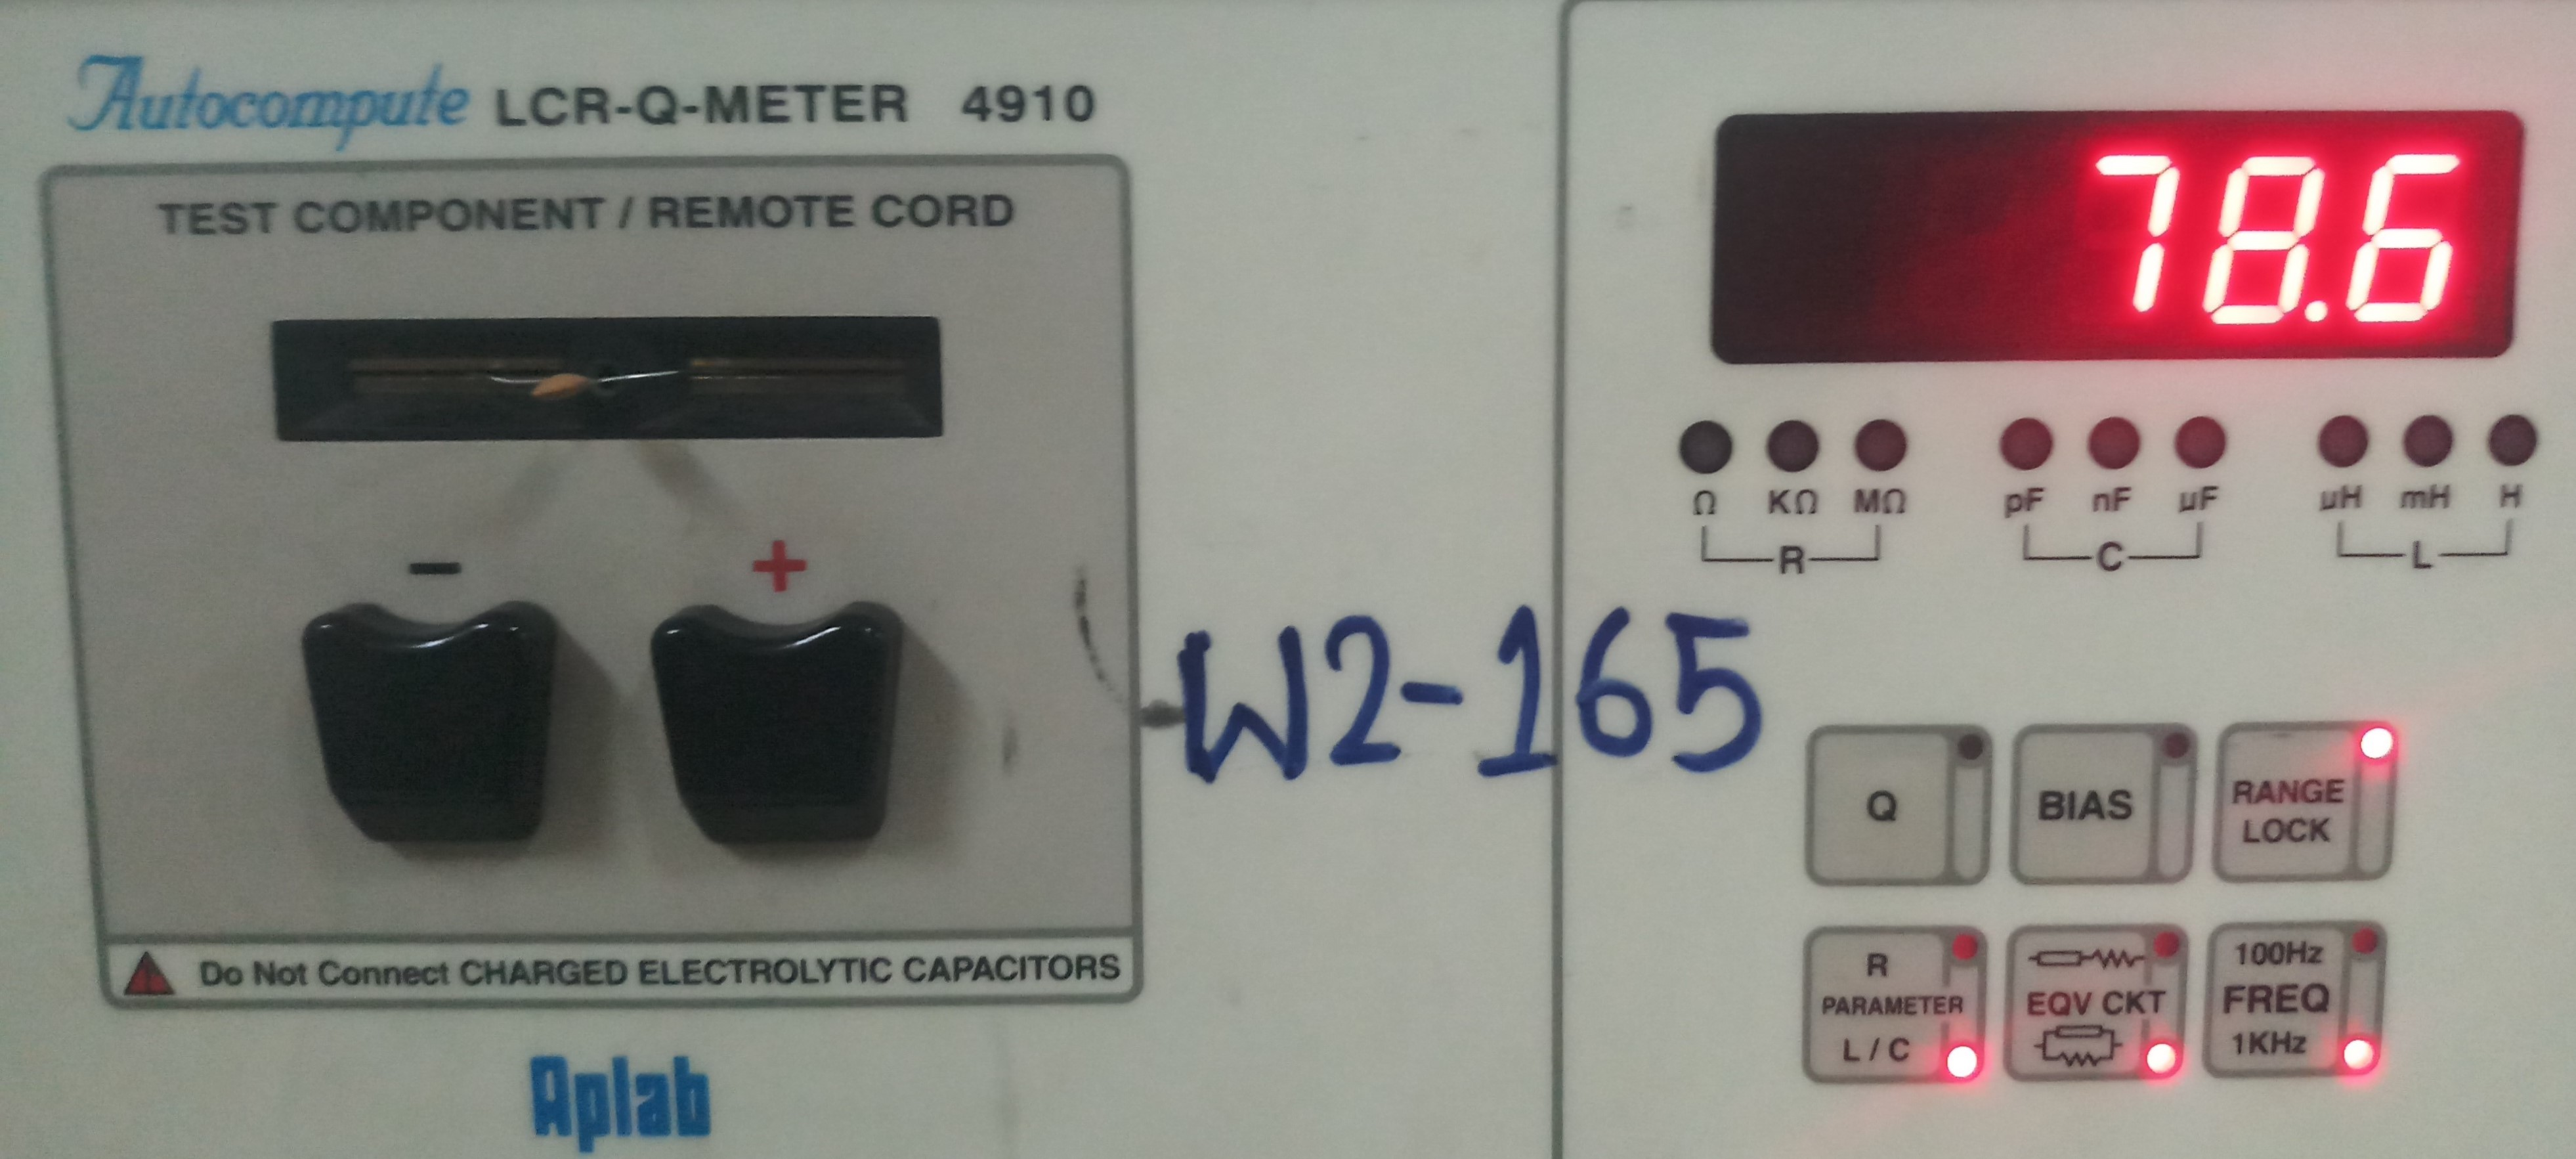
\includegraphics[scale=0.055]{RealCapacitance.jpg}
	\caption{Real Capacitance of the capacitor provided}
\end{figure}

\subsection{Part D}
Before calculating the capacitances, it is noteworthy to mention that we obtained the phase difference for one reading and the frequency used throughout. Though we could have used the phase difference in order to find the capacitance, we used the peak-to-peak amplitude since it was less hectic. As expected, the phase difference turns out to be around \( 90^{\circ} \).
\begin{figure}[H]
	\centering
	\begin{subfigure}[b]{0.475\linewidth}
		\centering
		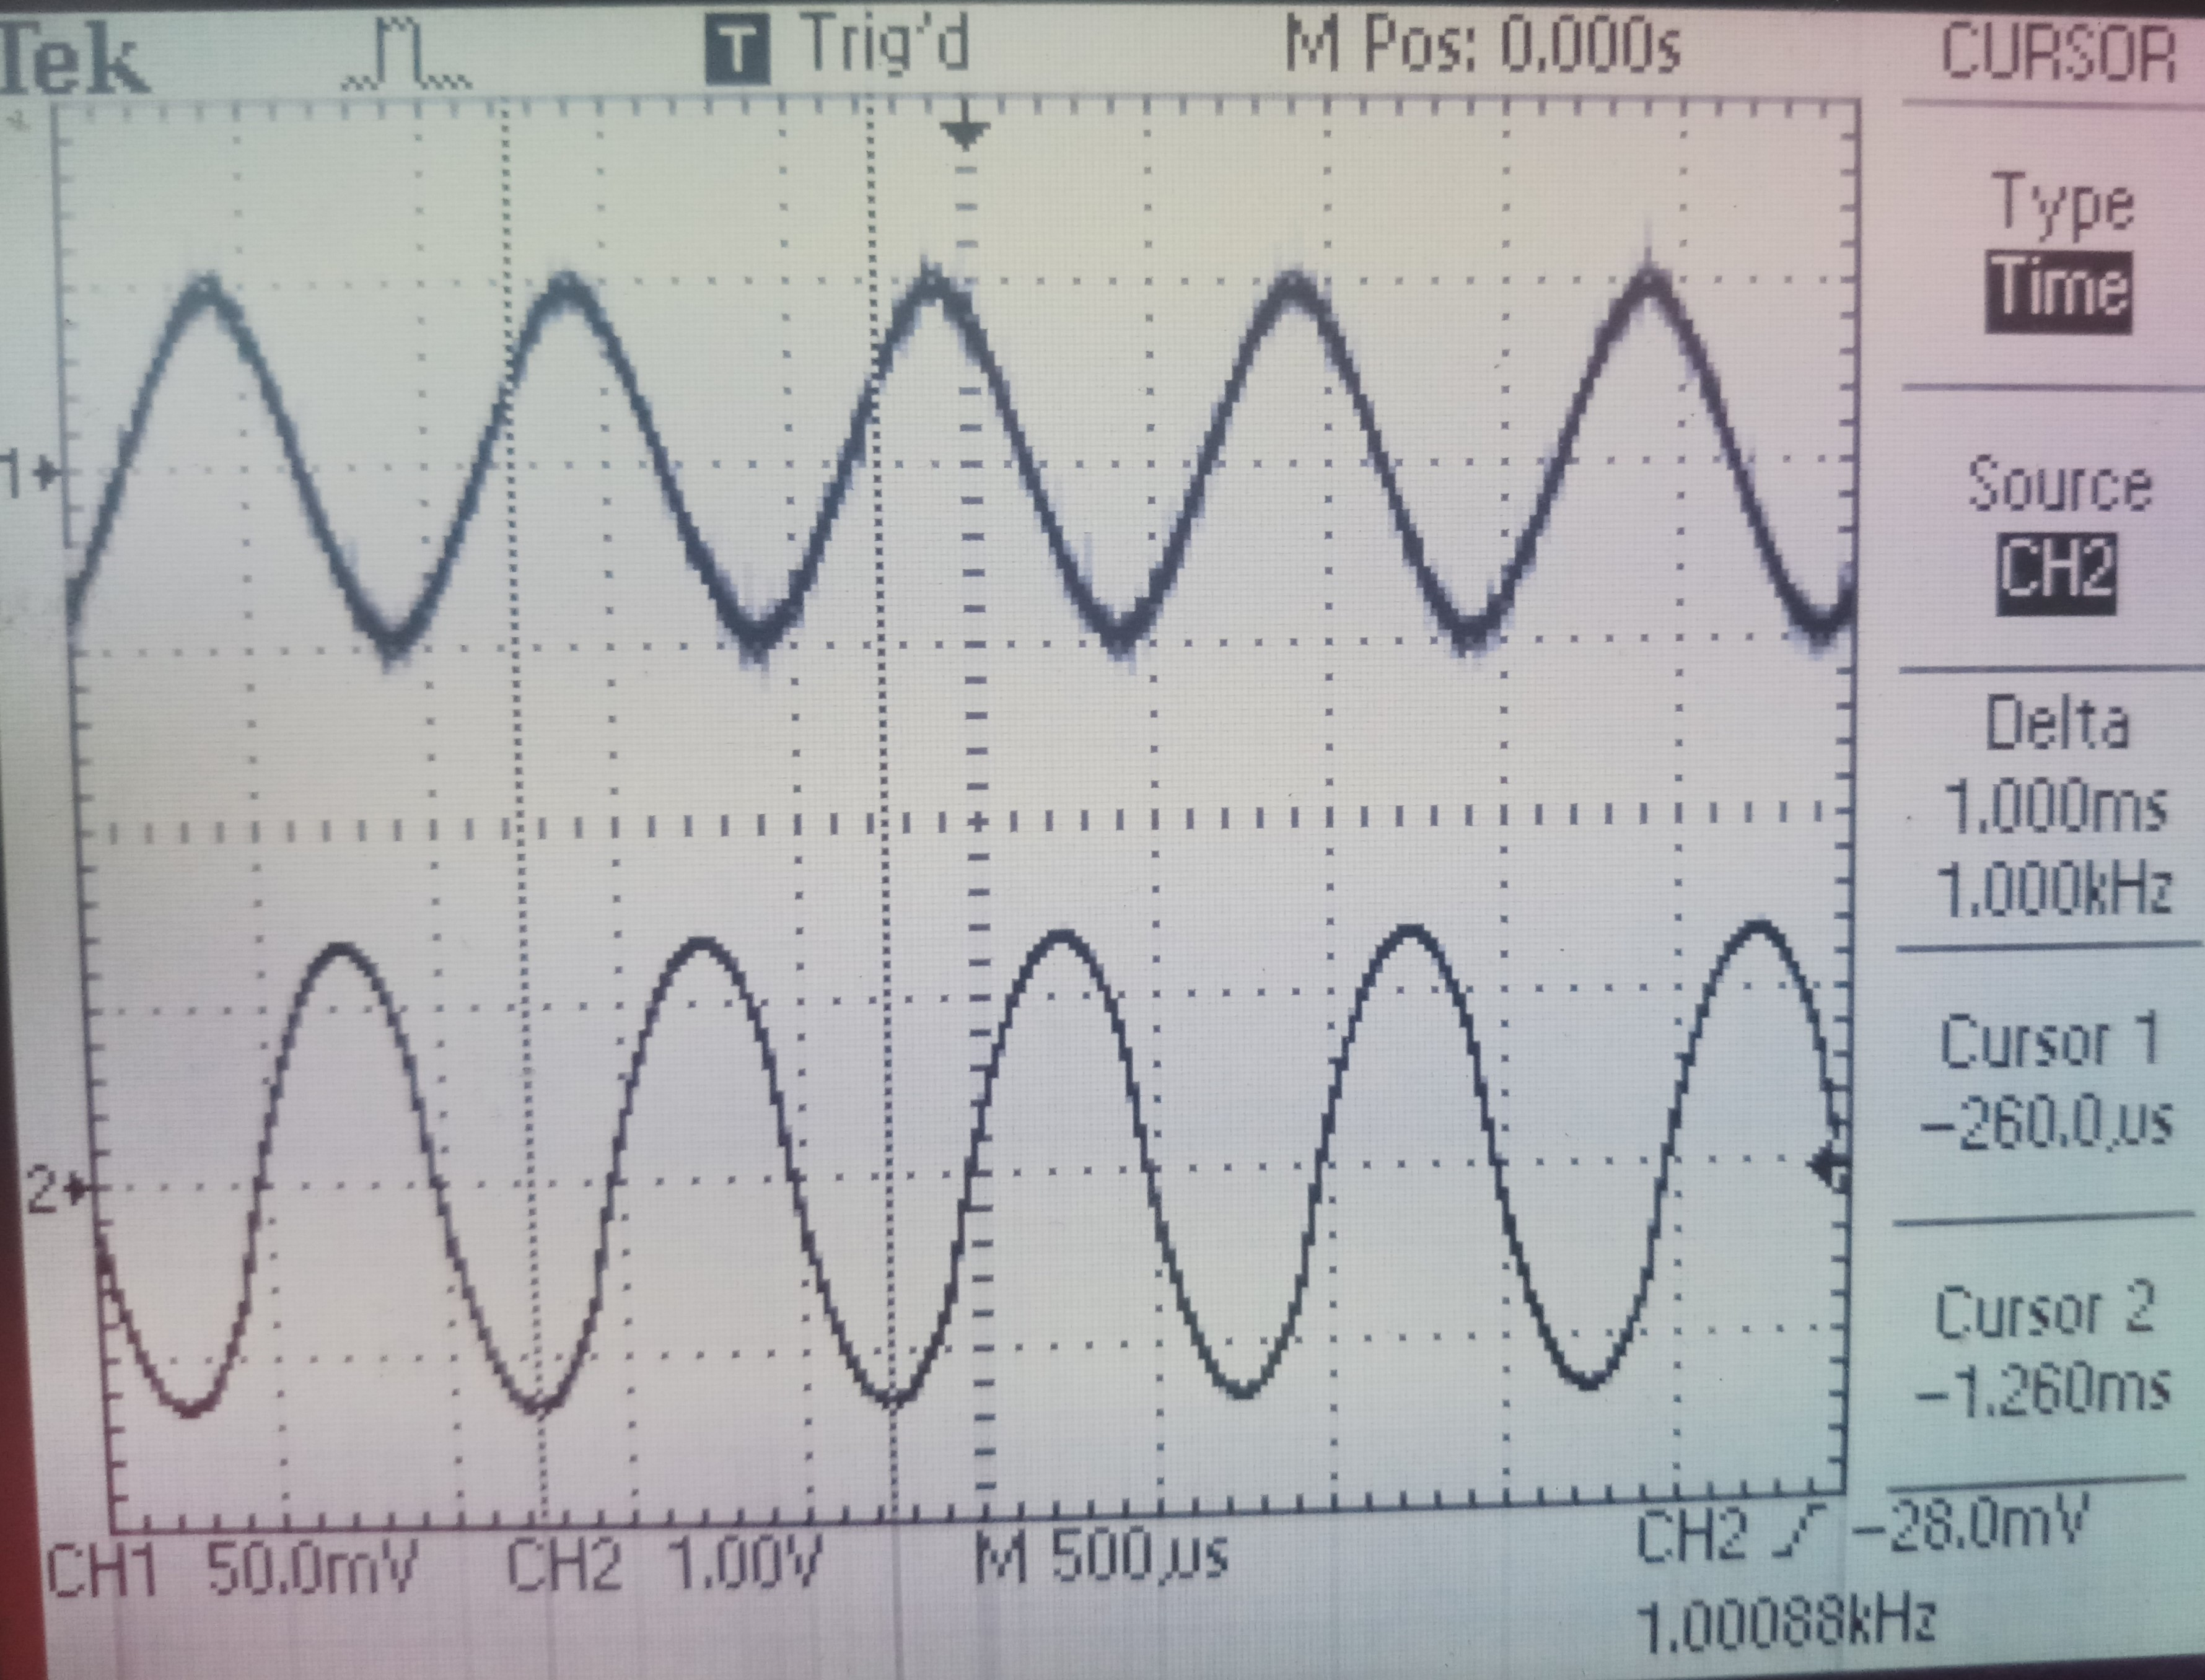
\includegraphics[width = \linewidth, trim = {0 0 0 0}, clip]{PartD_FreqMeasure.jpg}
		\caption{Frequency measurement (\( \approx 1kHz \))}
	\end{subfigure}
	\begin{subfigure}[b]{0.475\linewidth}
		\centering
		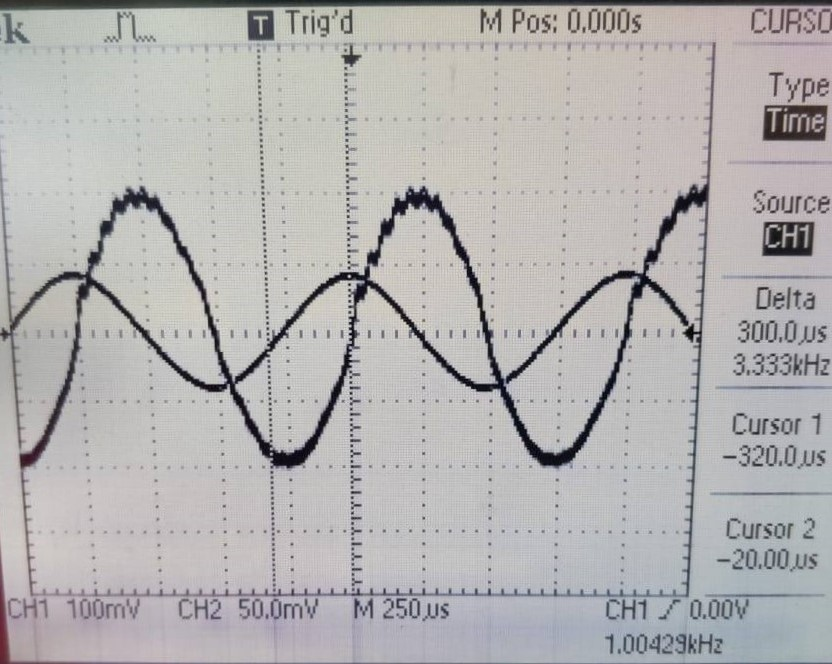
\includegraphics[width = \linewidth, trim = {0 0 0 0}, clip]{PartD_PhaseDiff.jpg}
		\caption{Measurement of Phase Difference}
	\end{subfigure}
	\caption{Part D - Initial Analysis}
\end{figure}
We use the same result as used in Part C:
\[ V_{out} = -V_{DUT}\left( \frac{Z_{fb}}{Z_{DUT}} \right) \] \[ C_{DUT} = \left( \frac{- V_{out_{p-p}}}{Z_{fb} \times \omega \times V_{DUT_{p-p}}} \right) \] \[ C_{DUT} = \left(  \frac{-V_{out_{p-p}}}{7723 \times 2 \pi \times \nu \times V_{DUT_{p-p}}} \right) \] \\
We obtain the following table by calculating the capacitance and the inverse of its square:
\begin{center}
 \begin{tabular}{||c | c | c ||} 
 \hline 
 \multicolumn{3}{||c||}{\( \nu \approx 1kHz \)} \\
 \hline
 \( V_{DC} \) & \( C \) & \( \frac{1}{C^2} \) \\
 \hline\hline
 0.1V & 184.47 nF & 0.000029387 \\
 0.3V & 156.46 nF & 0.000040850 \\
 0.4V & 141.18 nF & 0.000050171 \\
 0.5V & 135.82 nF & 0.000054209 \\
 0.8V & 119.59 nF & 0.000069921 \\
 1.0V & 109.43 nF & 0.000083508 \\
 1.2V & 108.13 nF & 0.000085528 \\
 \hline
\end{tabular}
\end{center}
For doing so, we used the following graphs and applied the equations obtained earlier:
\begin{figure}[H]
	\centering
	\begin{subfigure}[b]{0.45\linewidth}
		\centering
		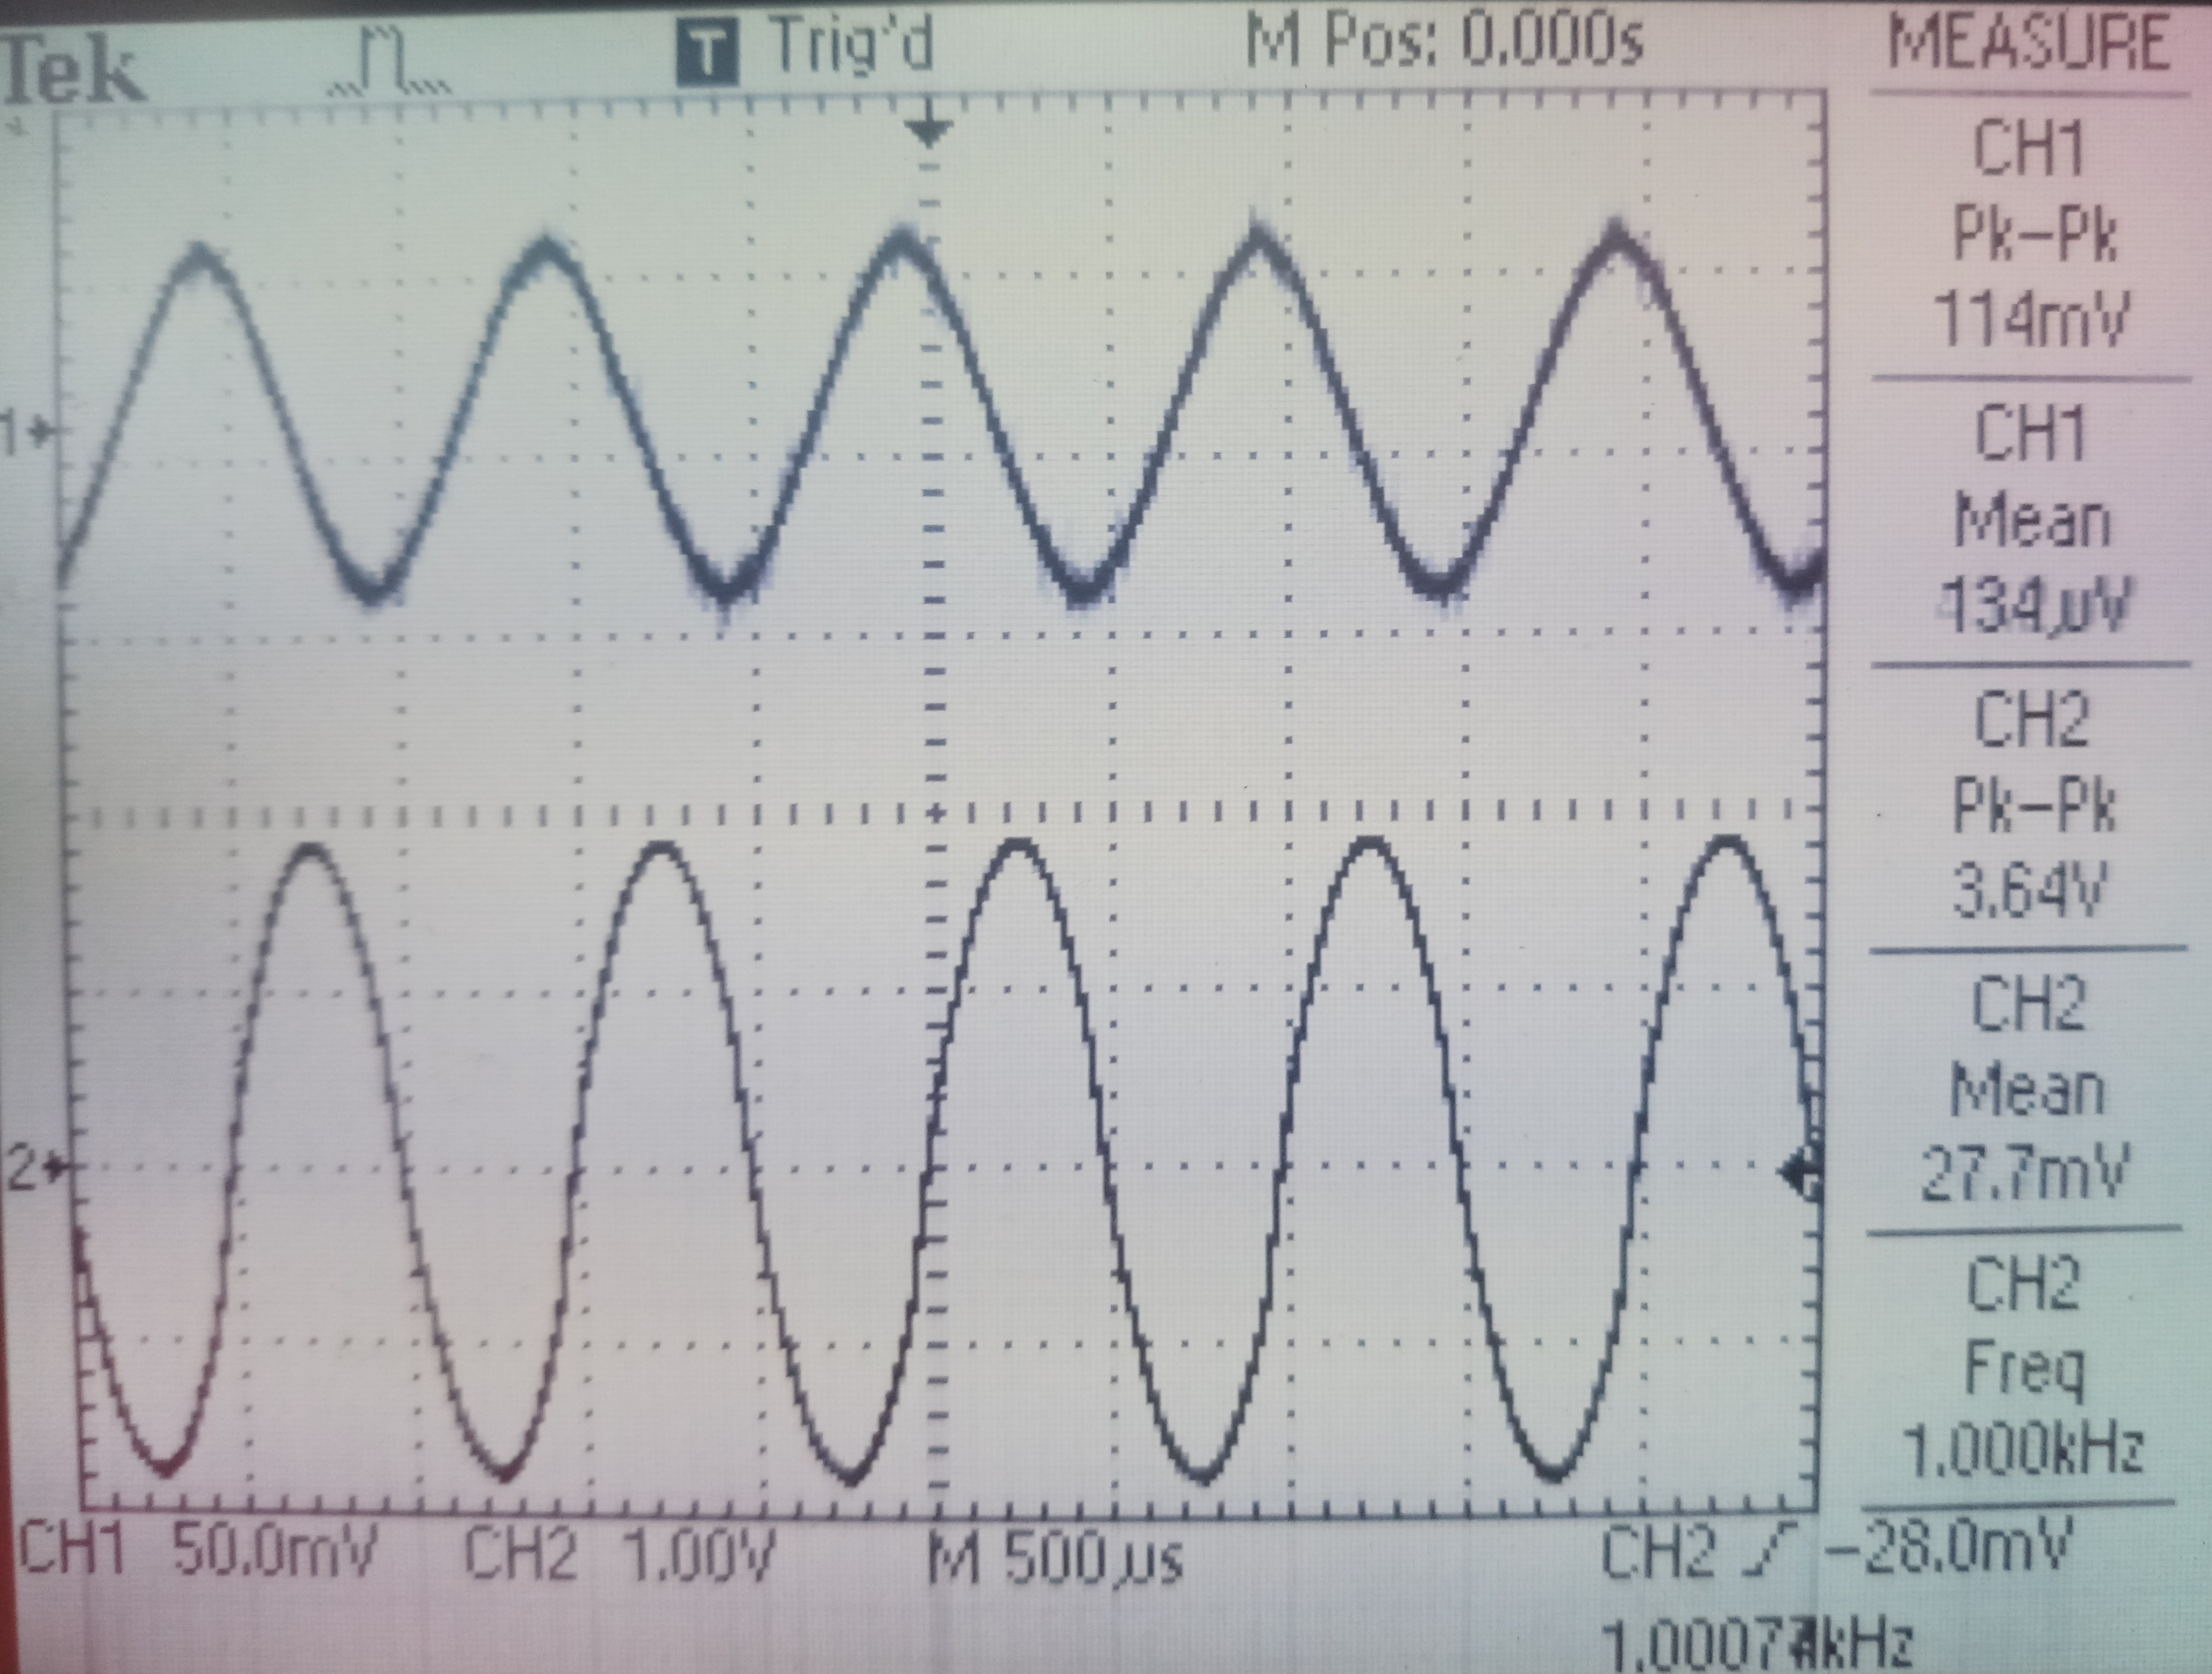
\includegraphics[width = \linewidth, trim = {0 0 0 0}, clip]{PartD_1.jpg}
		\caption{V = 0.1V}
	\end{subfigure}
	\begin{subfigure}[b]{0.45\linewidth}
		\centering
		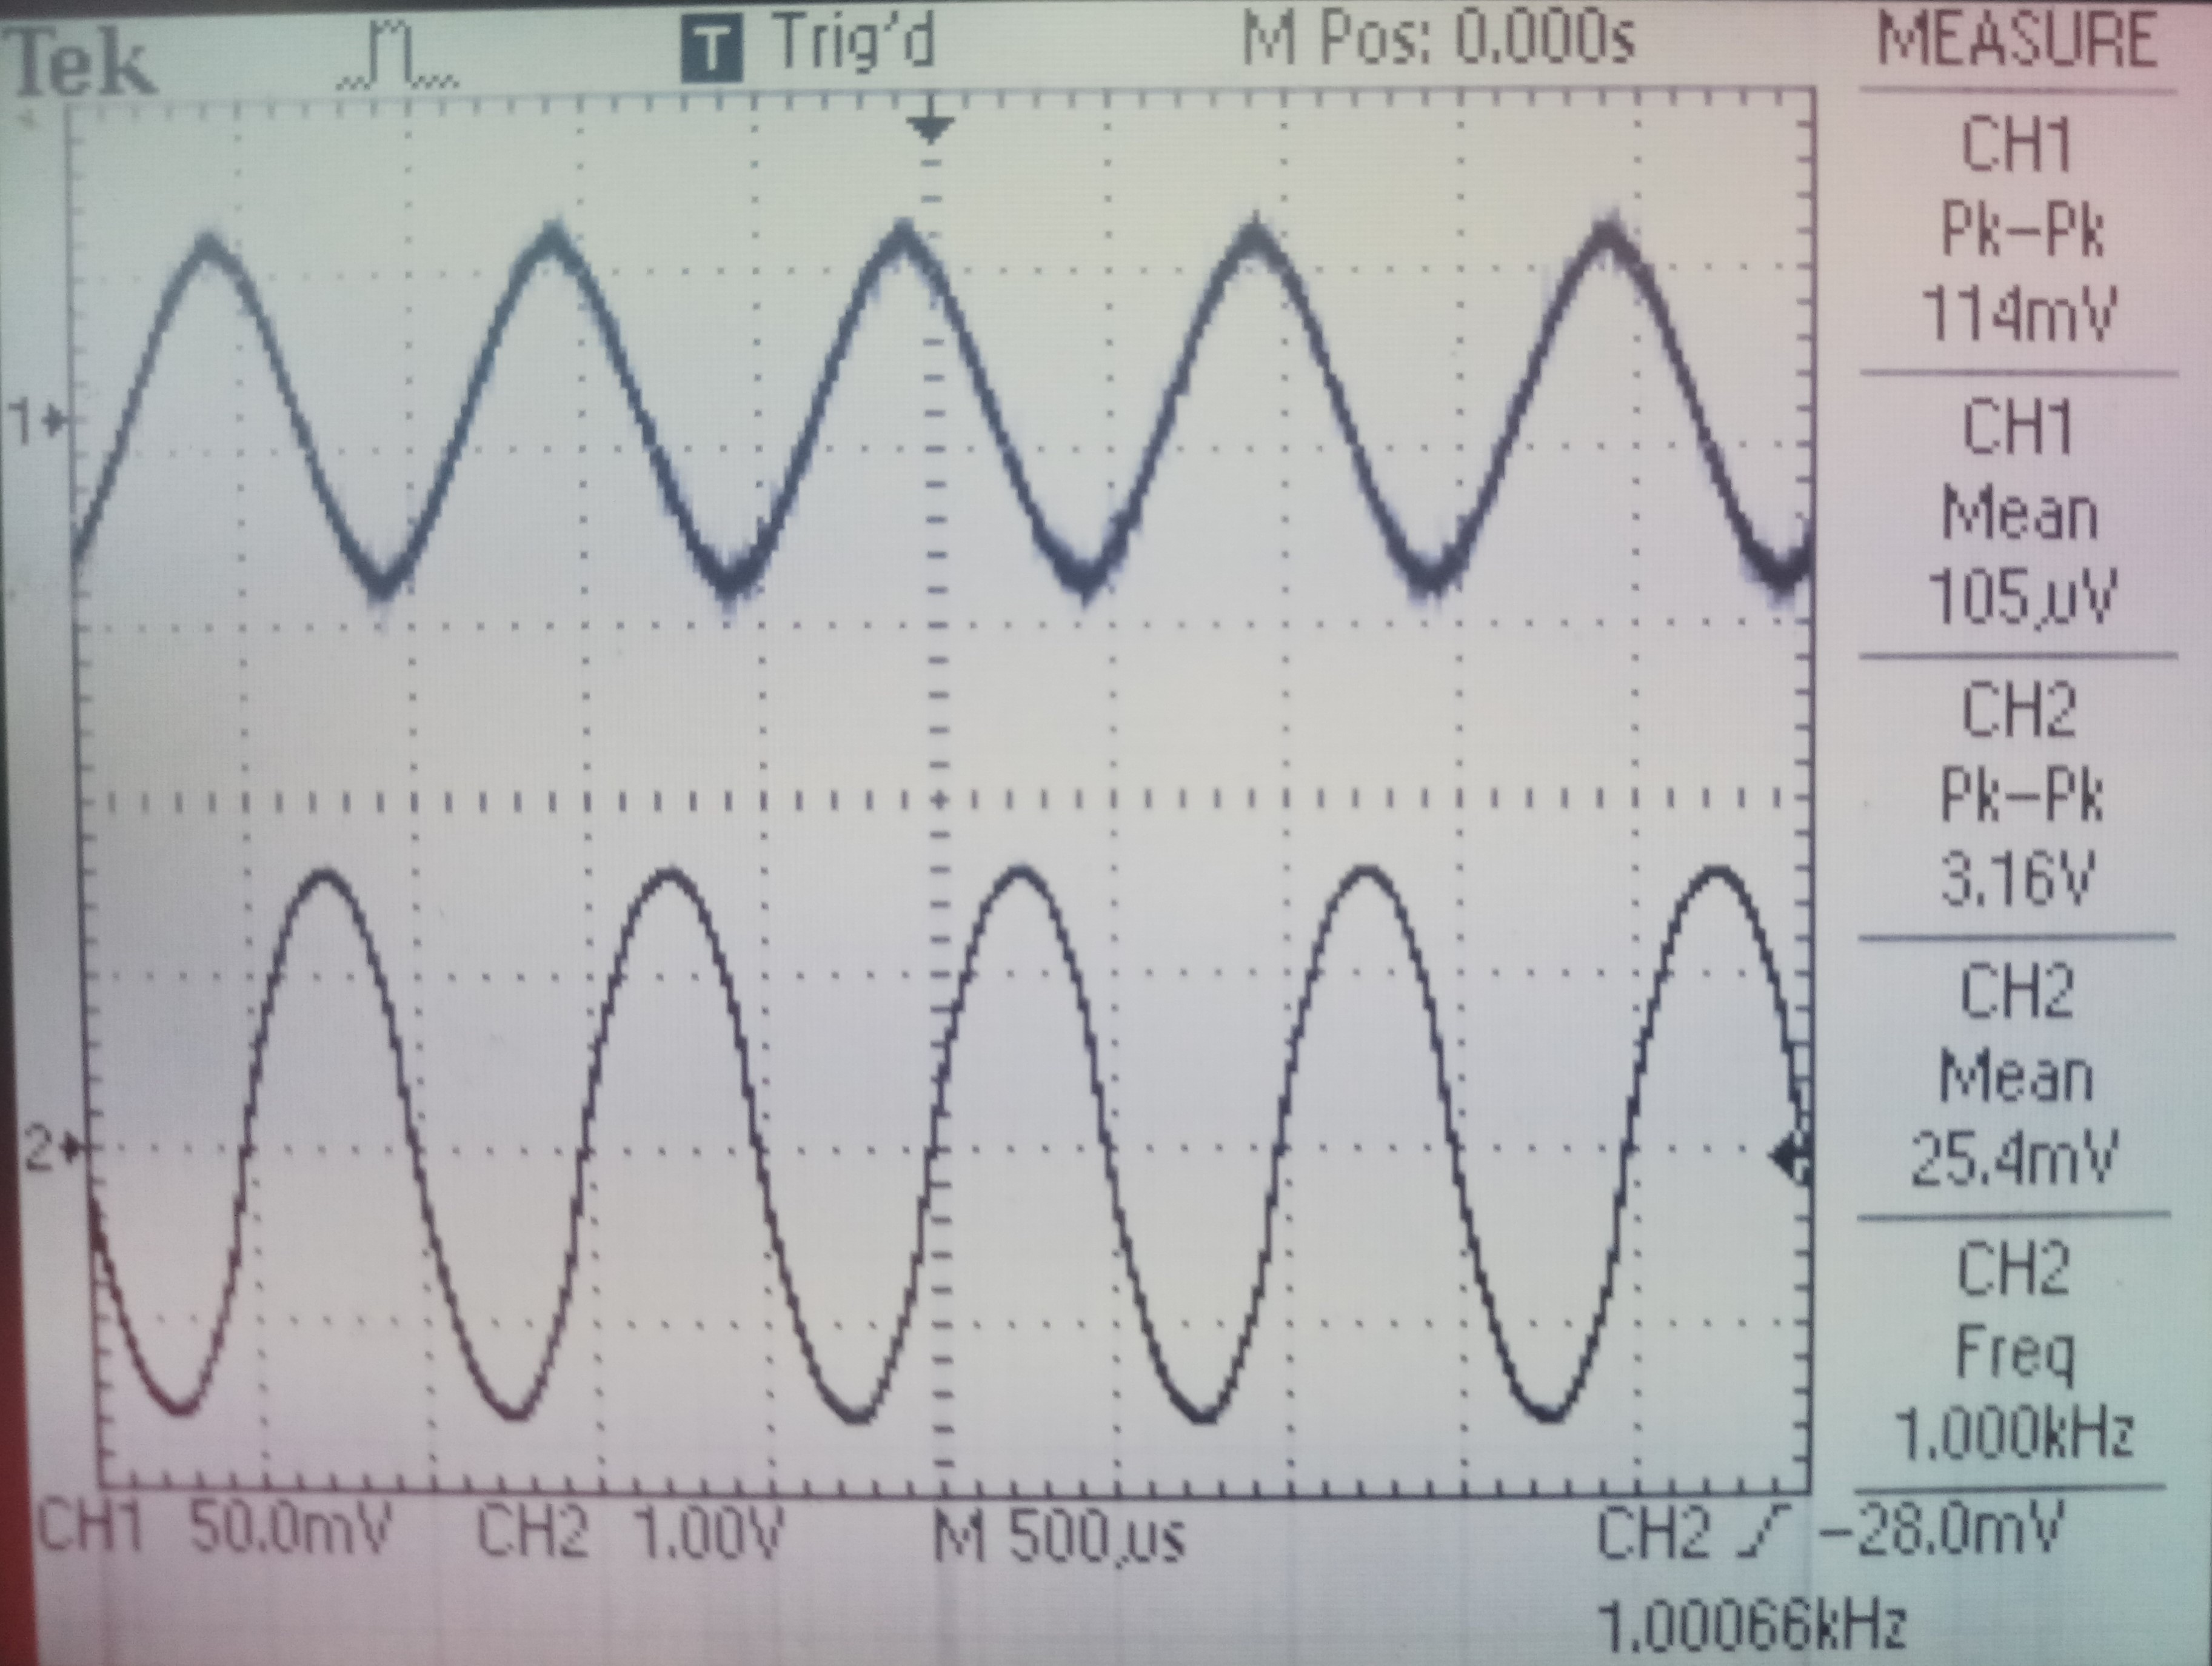
\includegraphics[width = \linewidth, trim = {0 0 0 0}, clip]{PartD_2.jpg}
		\caption{V = 0.3V}
	\end{subfigure}
	\begin{subfigure}[b]{0.45\linewidth}
		\centering
		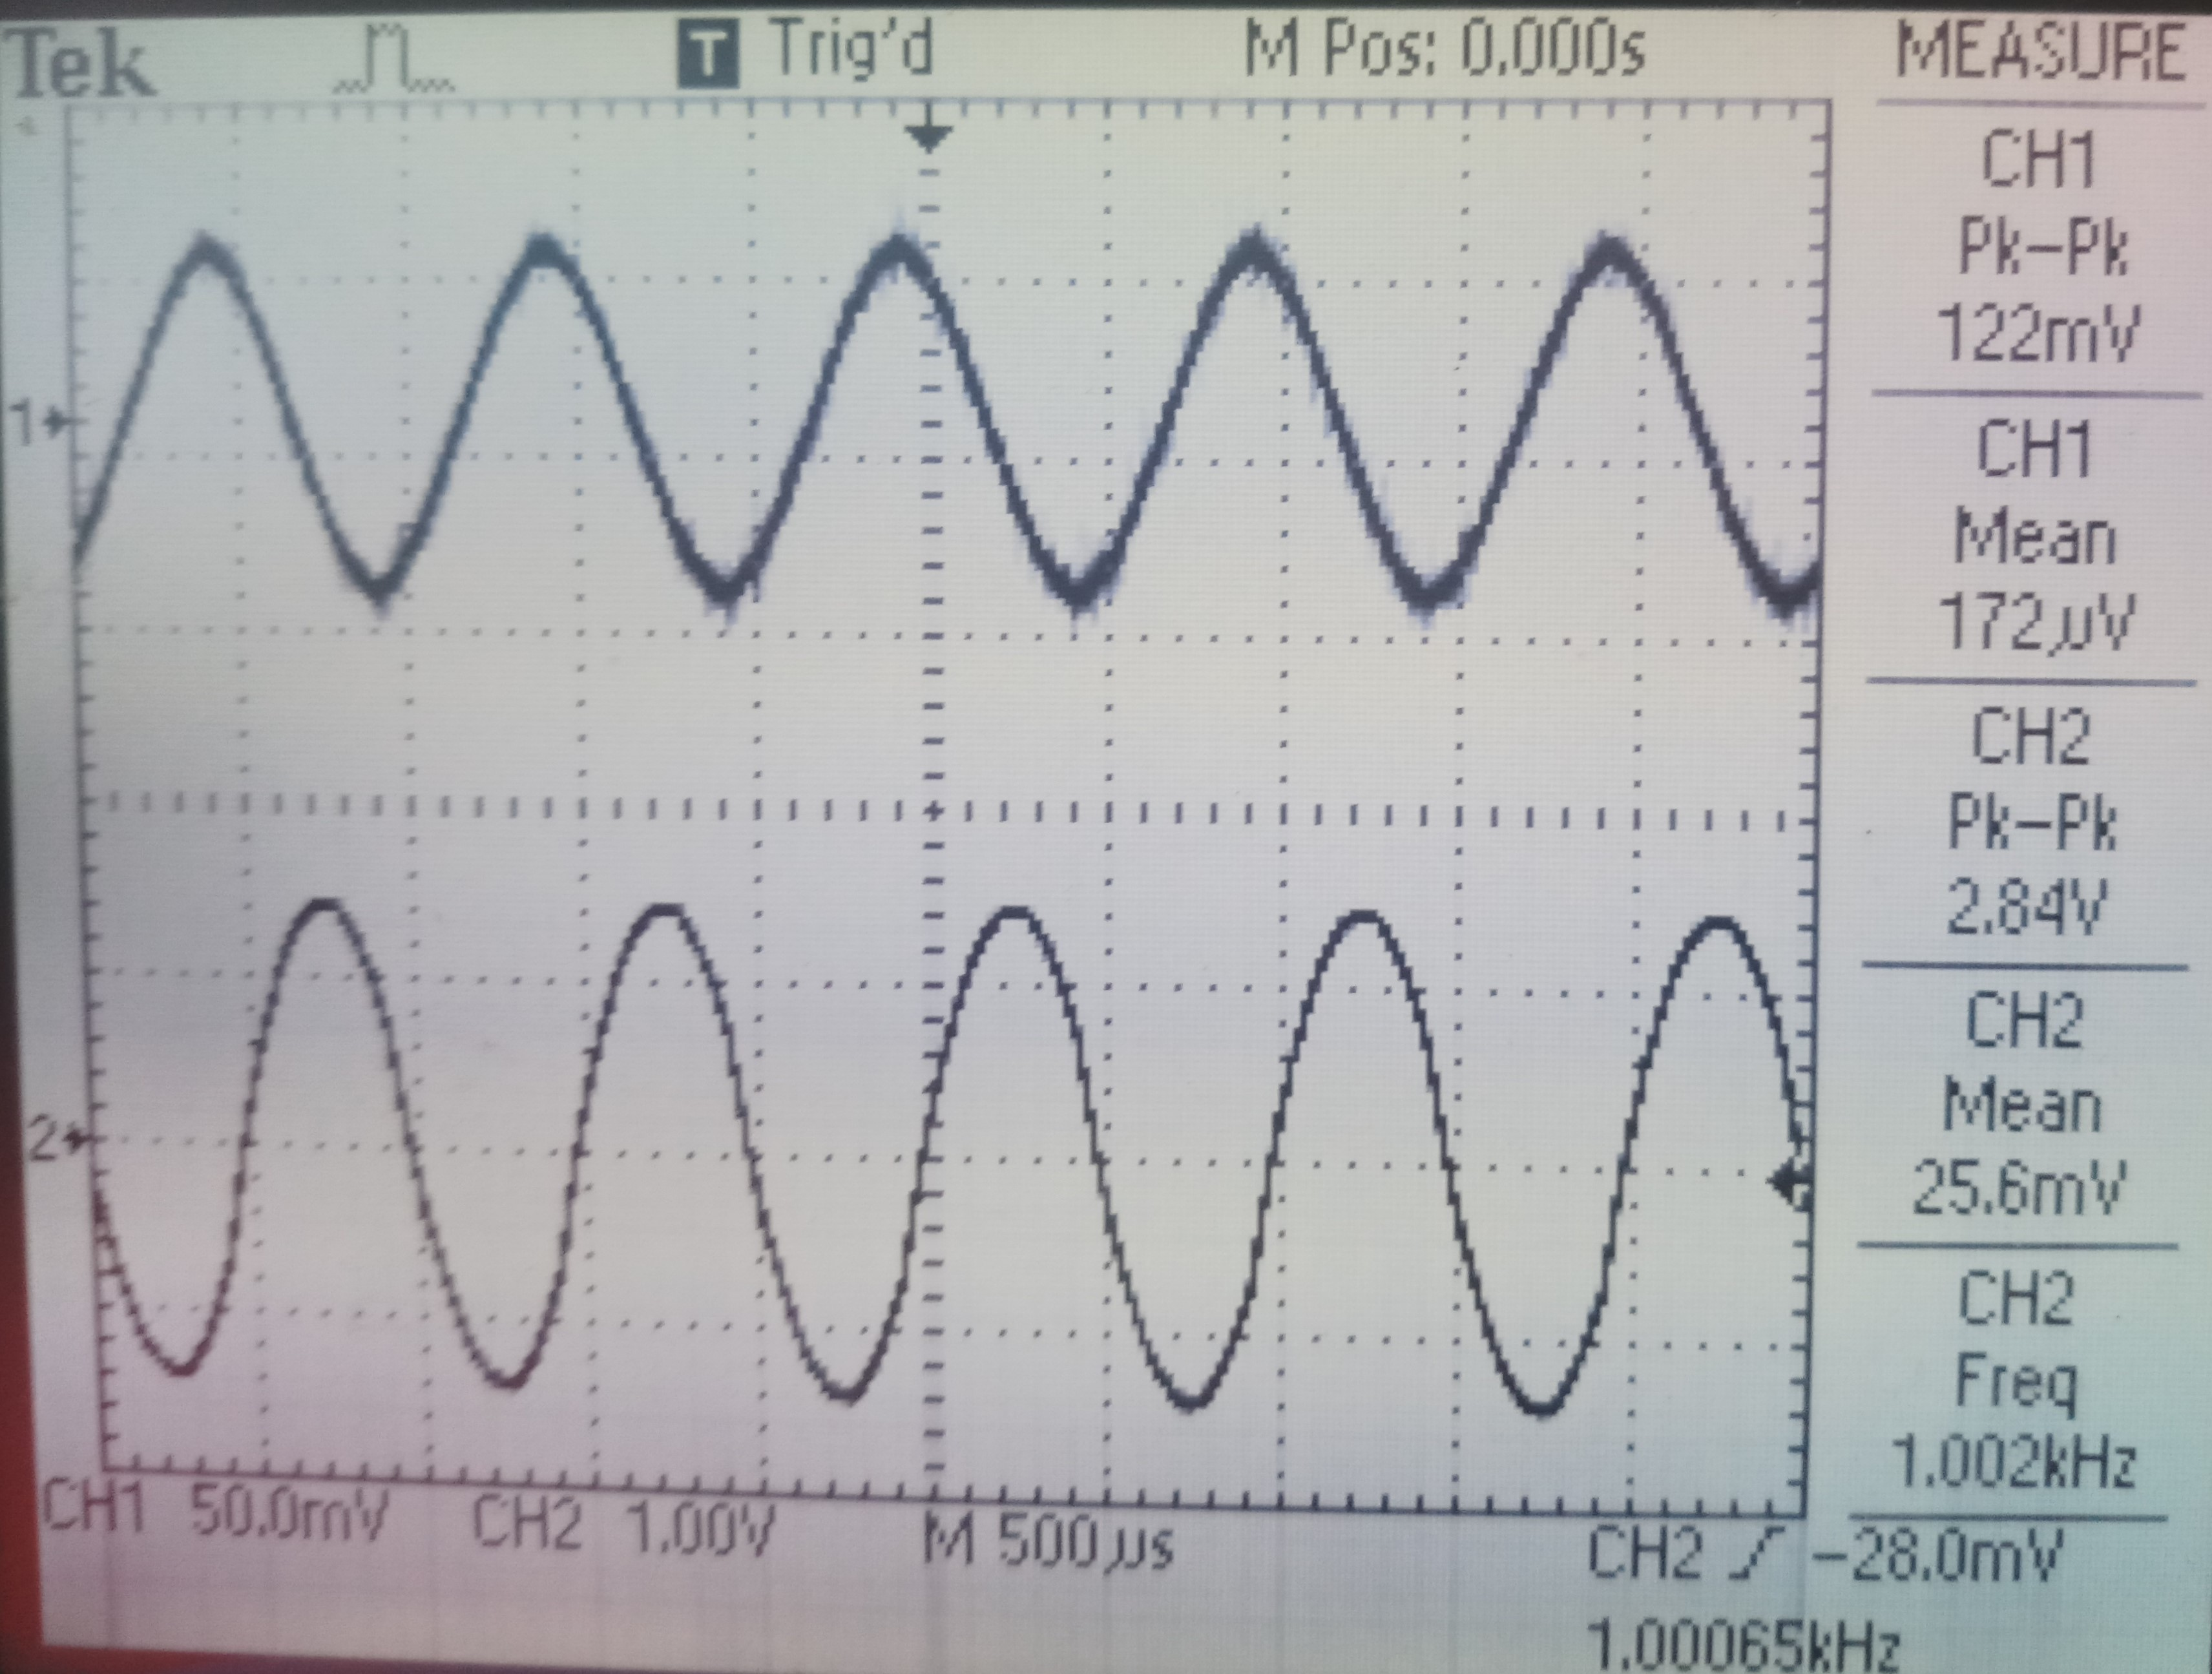
\includegraphics[width = \linewidth, trim = {0 0 0 0}, clip]{PartD_3.jpg}
		\caption{V = 0.4V}
	\end{subfigure}
	\begin{subfigure}[b]{0.45\linewidth}
		\centering
		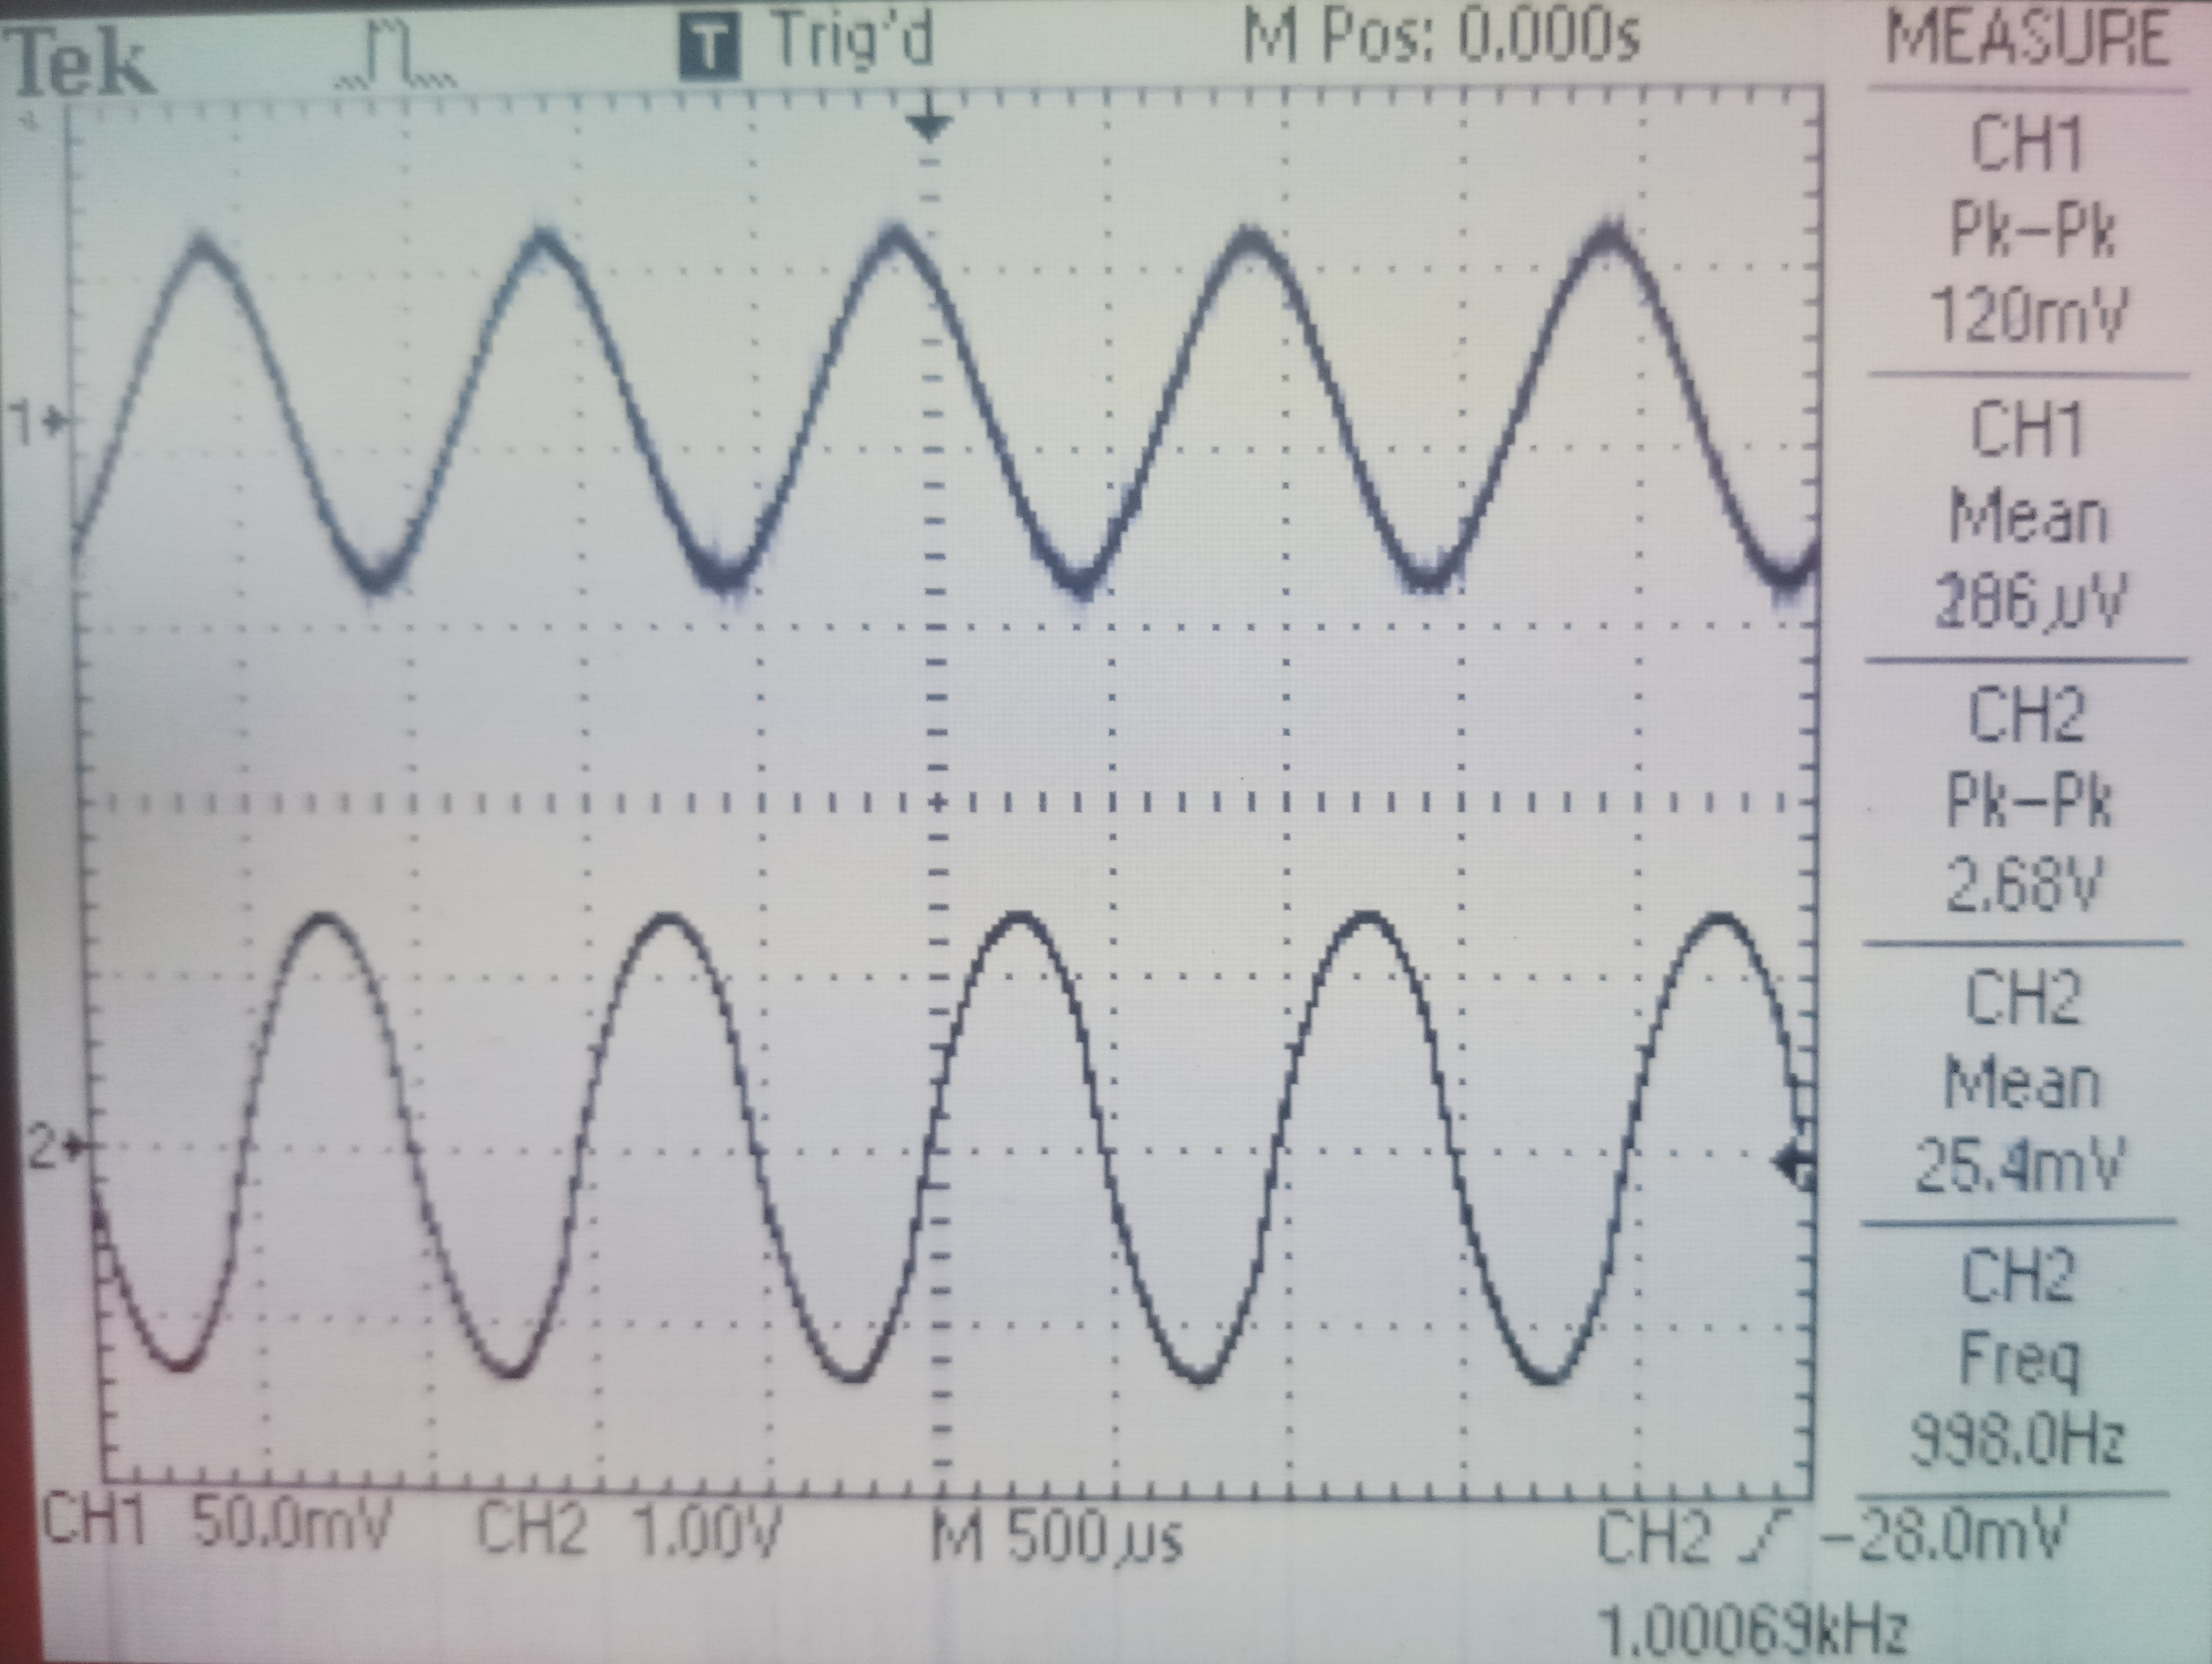
\includegraphics[width = \linewidth, trim = {0 0 0 0}, clip]{PartD_4.jpg}
		\caption{V = 0.5V}
	\end{subfigure}
	\begin{subfigure}[b]{0.45\linewidth}
		\centering
		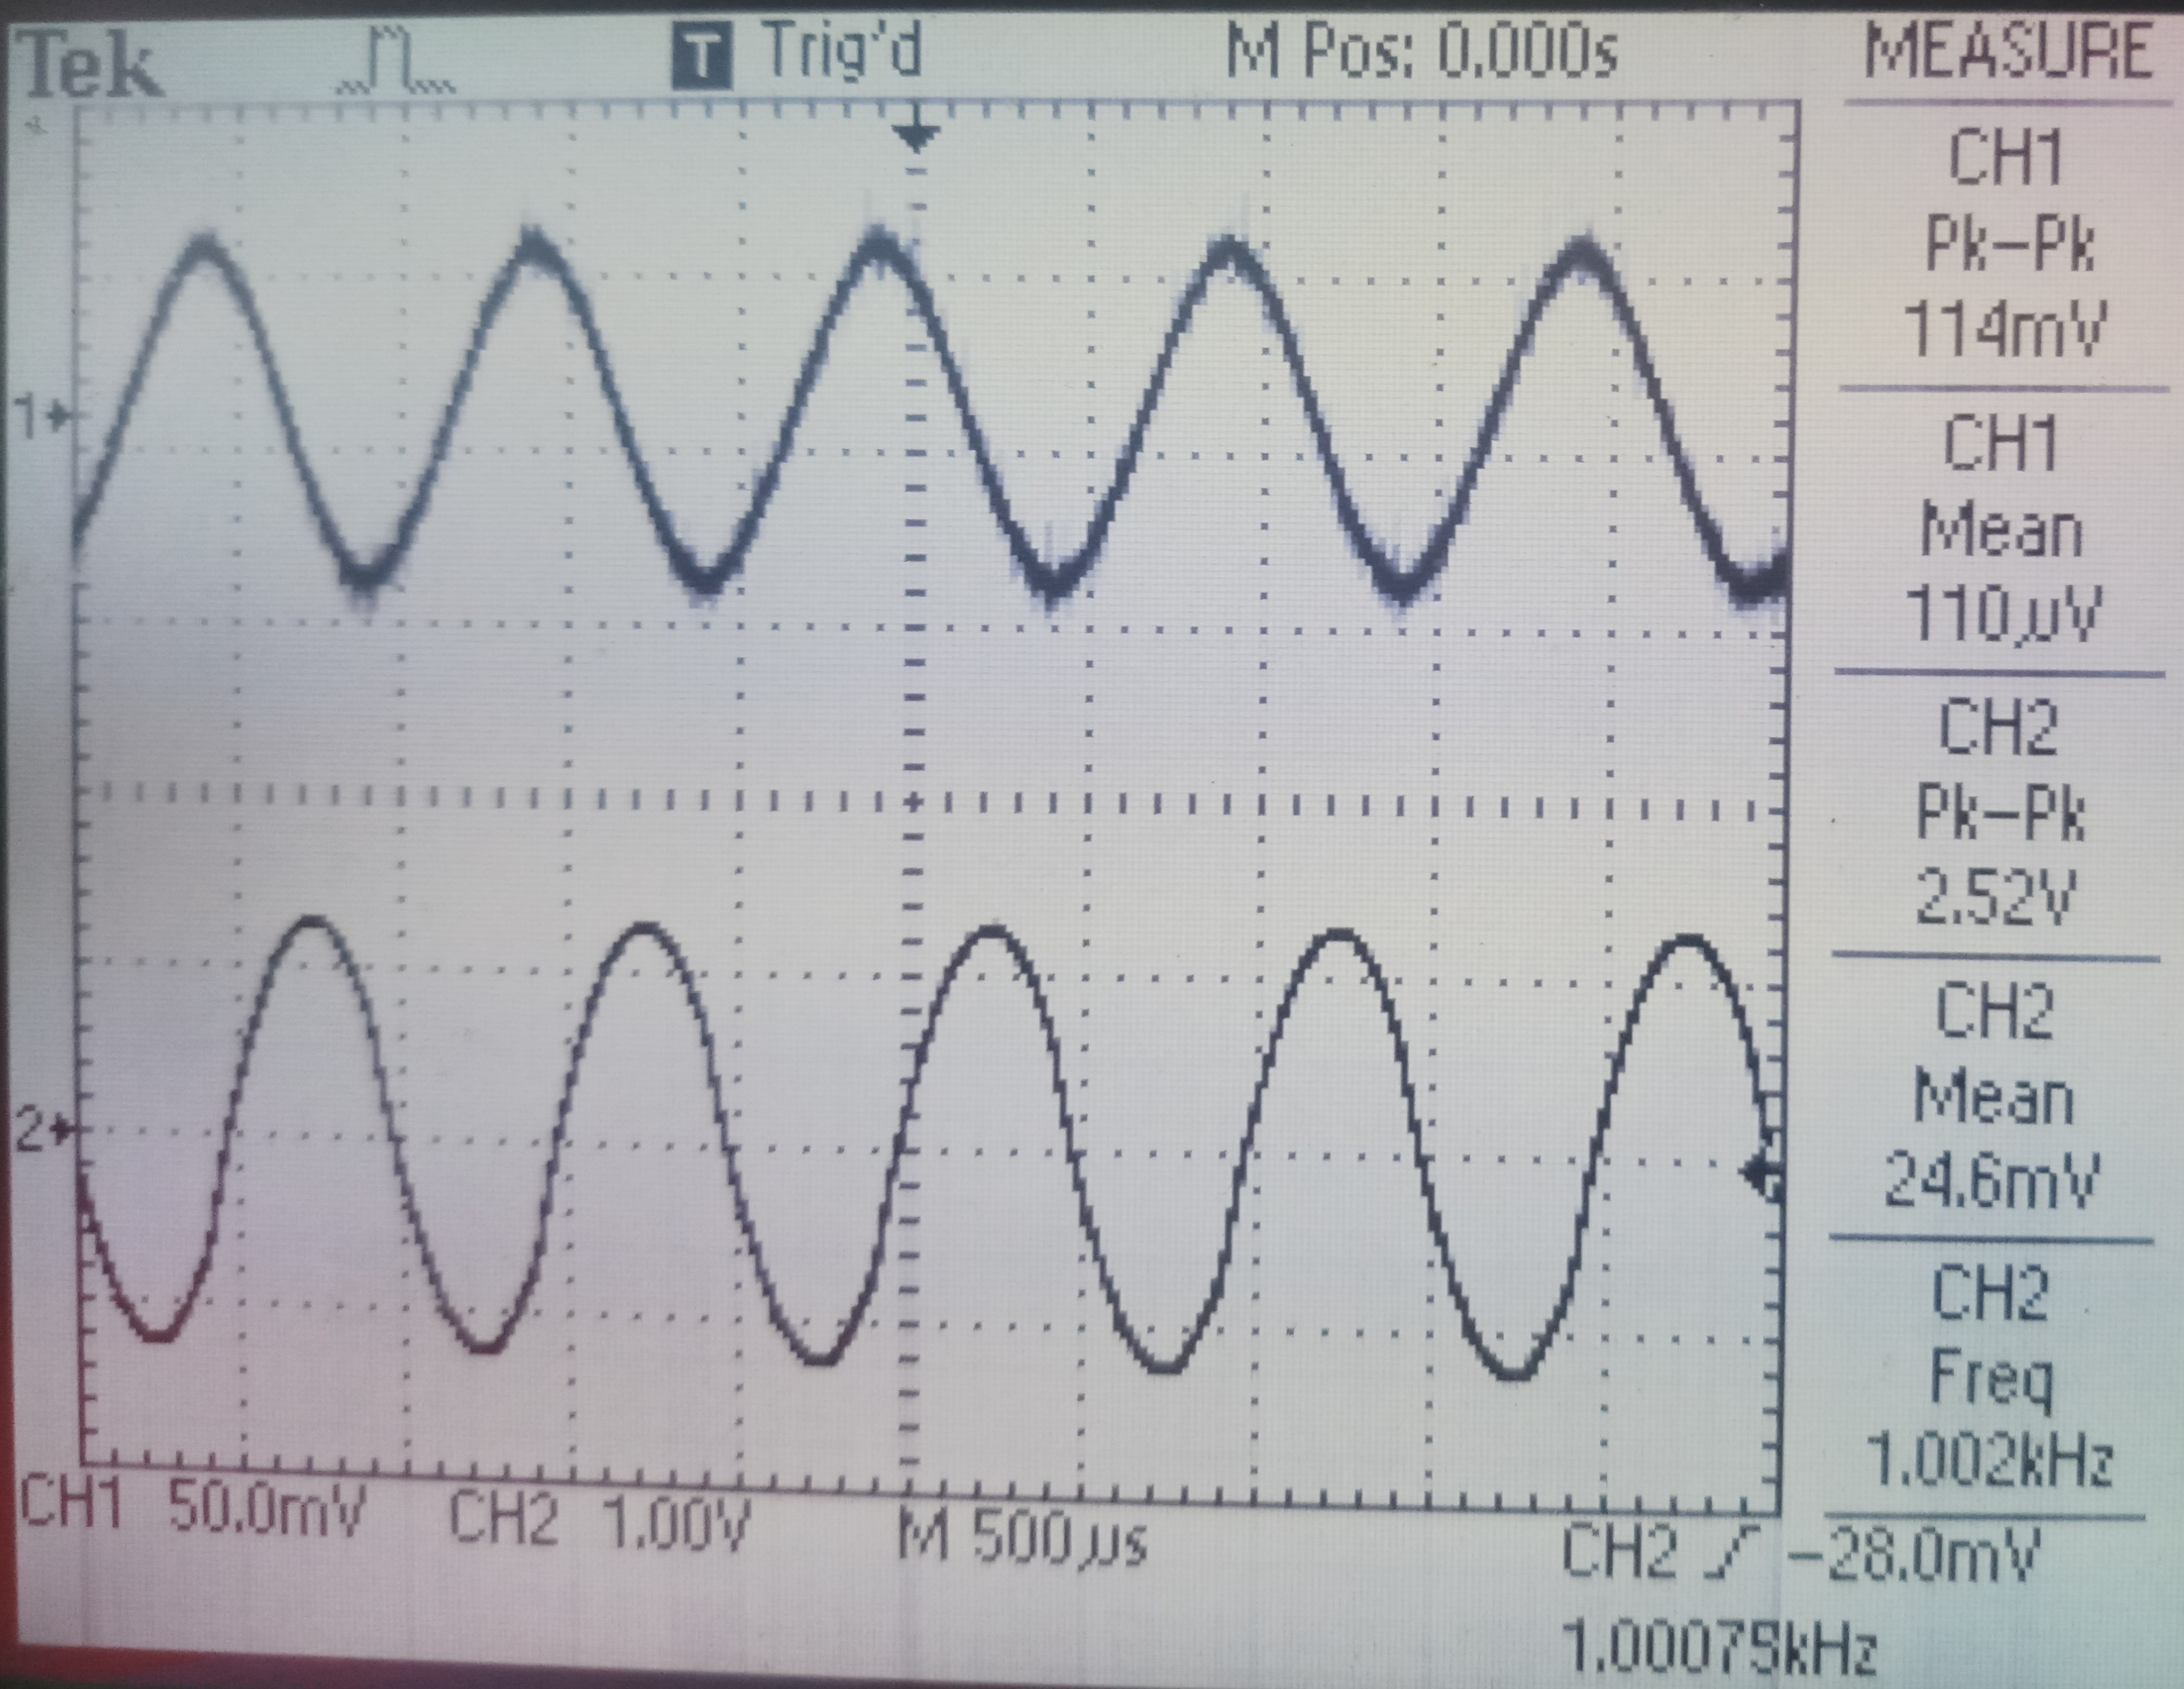
\includegraphics[width = \linewidth, trim = {0 0 0 0}, clip]{PartD_5.jpg}
		\caption{V = 0.8V}
	\end{subfigure}
	\begin{subfigure}[b]{0.45\linewidth}
		\centering
		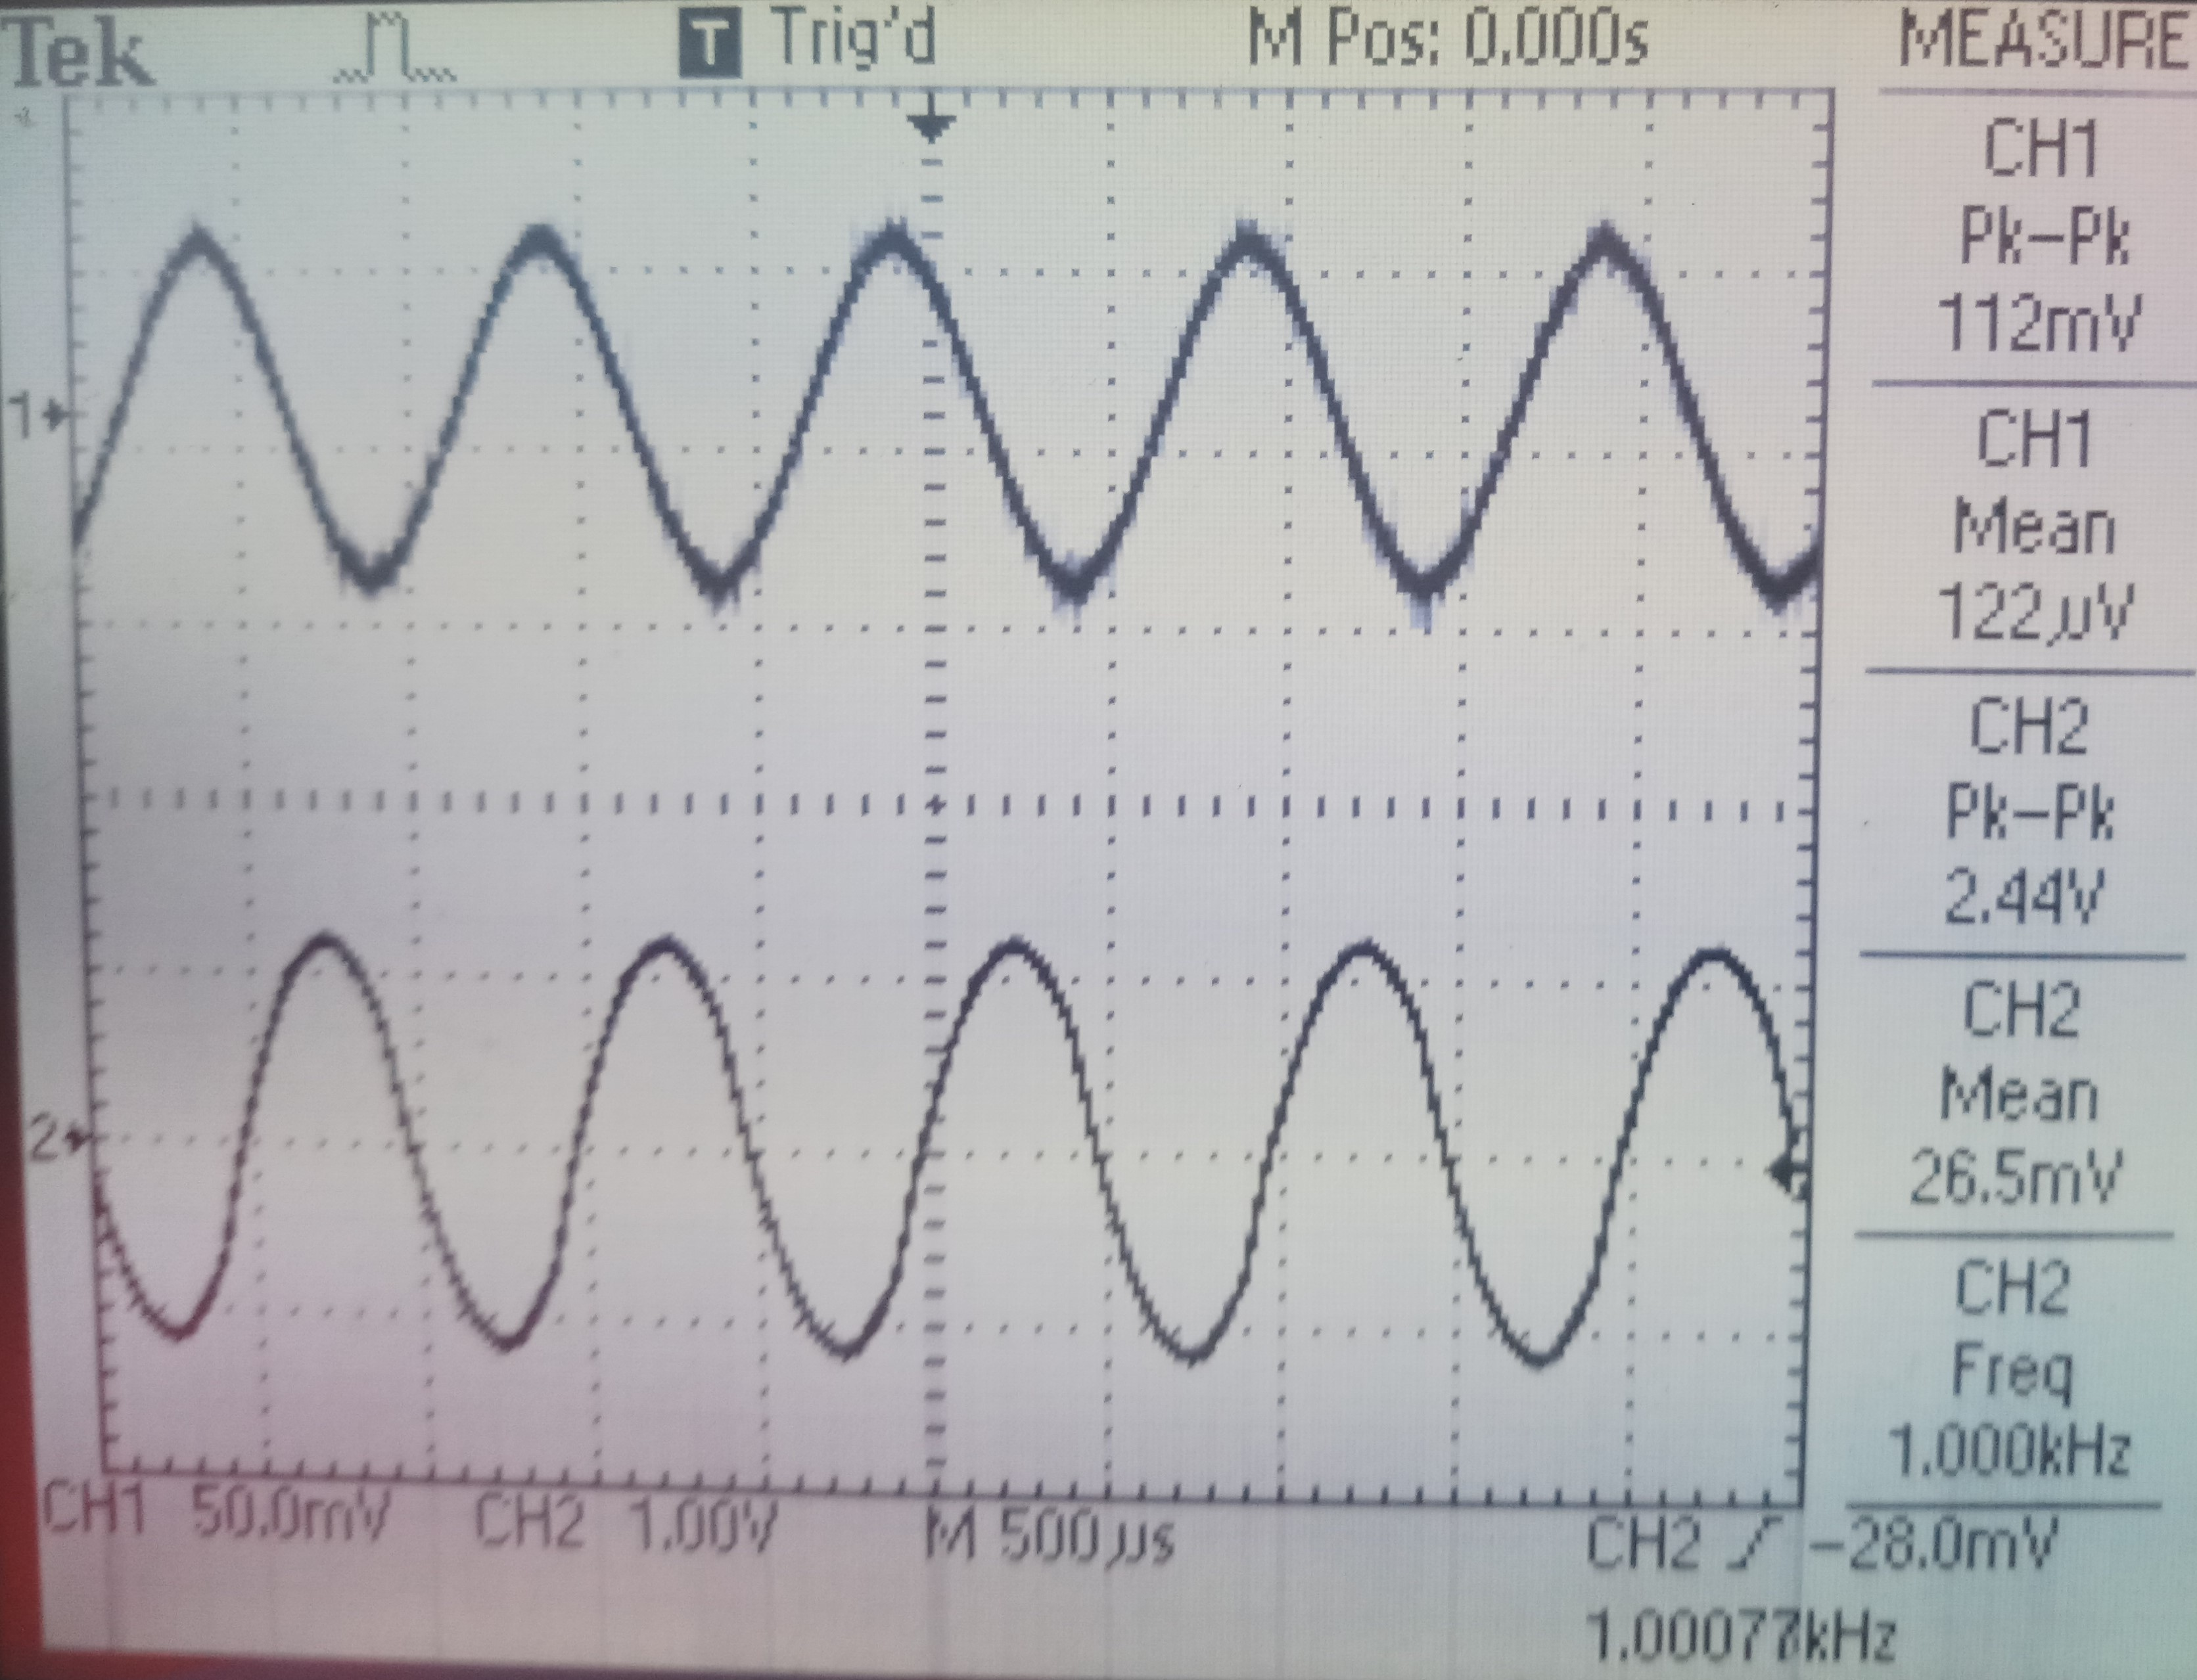
\includegraphics[width = \linewidth, trim = {0 0 0 0}, clip]{PartD_6.jpg}
		\caption{V = 1.0V}
	\end{subfigure}
	\begin{subfigure}[b]{0.45\linewidth}
		\centering
		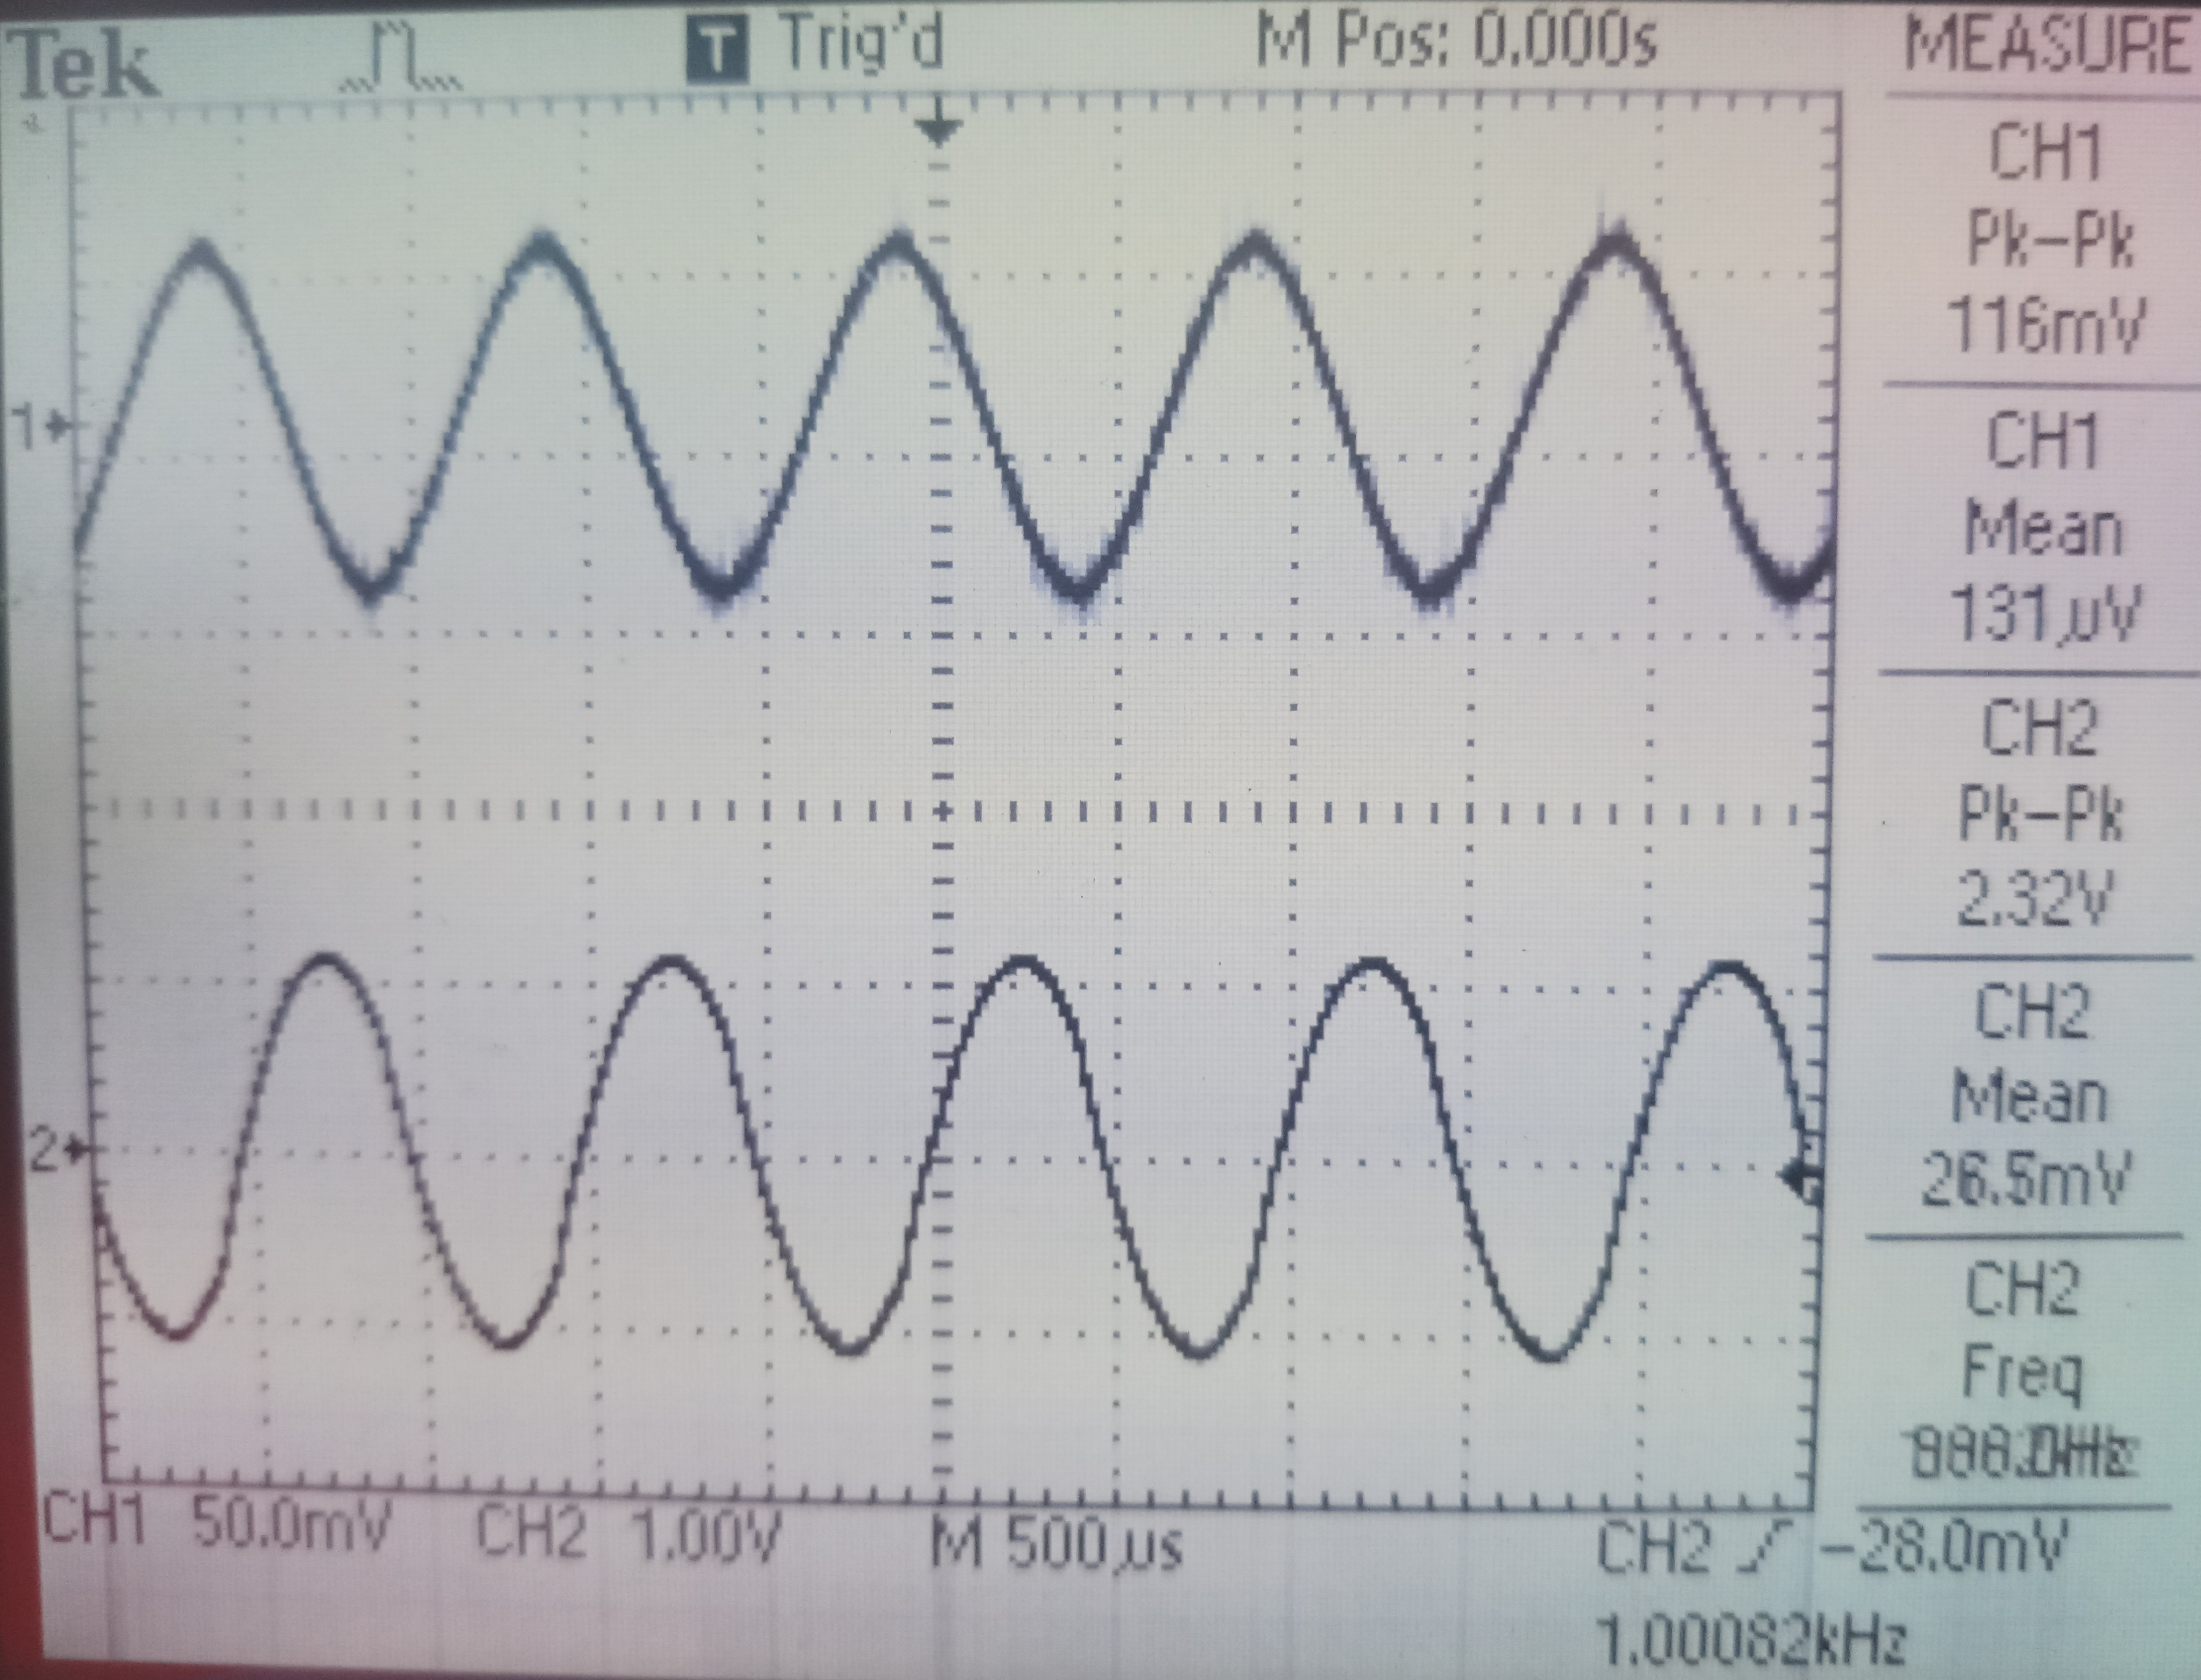
\includegraphics[width = \linewidth, trim = {0 0 0 0}, clip]{PartD_7.jpg}
		\caption{V = 1.2V}
	\end{subfigure}
	\caption{Part D - Values of output for \( \nu \approx 1kHz\)}
\end{figure}
On plotting these values, we get the following curve:
\begin{figure}[H]
	\centering
	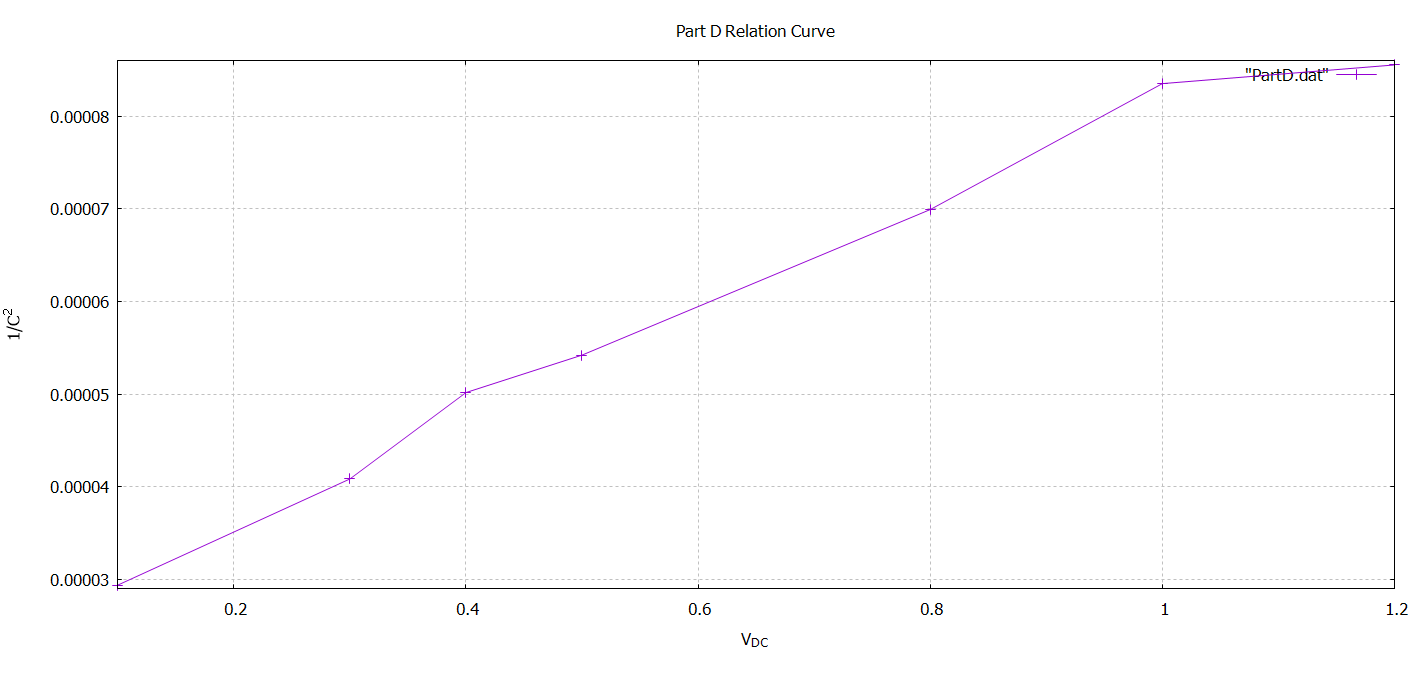
\includegraphics[scale=0.5]{RelationCurve.png}
	\caption{\( \frac{1}{C^2}\ vs\ V_{DC} \) curve}
\end{figure}

As is visible and was expected, the \( \frac{1}{C^2}\ vs\ V_{DC} \) curve is almost linear is nature.

The slope is given by \( \frac{d(\frac{1}{C^2})}{dV} = \frac{2}{q\epsilon_0\epsilon_sA^2N_d} \) which gives us the doping density \( N_d \) as:
\[ N_d = \frac{2}{q\epsilon_0\epsilon_sA^2\frac{d(\frac{1}{C^2})}{dV}} \]
Similarly, the built-in potential \( V_{bi} \) can be calculated from the x-axis intercept \( -V_{bi} \) or the y-axis intercept  \( \frac{2V_{bi}}{q\epsilon_0\epsilon_sA^2N_d} \). \\

Our obtained graph is best fit as \( y = (2.65 + 5.31x) \times 10^{-5} \). Hence we get the built-in voltage as the negative of the x-axis intercept; i.e. \[ V_{bi} = \frac{-(-2.65)}{5.31} = 0.499 \approx 0.5V \] \\
In all our calculations, \( \frac{1}{C^2} \) was in the units of \( nF^{-2} \). Hence we get the doping density given by the above formula: \[ N_d = 10^{-18} \times \frac{2}{q\epsilon_0\epsilon_sA^2\frac{d(\frac{1}{C^2})}{dV}}\] \[ N_d = 10^{-18} \times \frac{2}{(1.6 \times 10^{-19}) \times (8.854 \times 10^{-12}) \times (11.7) \times (1.6 \times 10^{-3})^2 \times (5.31 \times 10^{-5})} \] \[ N_d = 8.88 \times 10^{20} m^{-3} = 8.88 \times 10^{14} cm^{-3} \]

\section{Reflection questions}

1. You have worked with Schottky barrier diodes in previous lab. Would a reverse biased Schottky barrier's capacitance measurement allow you to infer certain properties of the semiconductor? What may be the advantages of using a Schottky diode over a pn junction diode?\\
Ans. The speed of the diode is way faster and it is easier to use the diode. Moreover the values obtained are higher in value hence reducing the effect of noise.\\

2. In this experiment, you measured the capacitance of a pn junction to estimate the doping density of silicon. The doping density can also be estimated by measuring the conductivity (or its inverse, the resistivity) of the wafer. You are probably familiar with the expression $R=\rho\frac{l}{A}$ for resistance expressed in terms of resistivity. How would you measure the resistivity of a silicon wafer? Would the same formula be useful?\\
Ans. The four-probe measurement system can be used to measure the resistivity.\\

\end{document}
